% =============================================================================
\subsection{Fase 1: Investigação Canônica dos Parâmetros}
\label{sec:fase1}

Esta fase segue o guia do enunciado no \code{synth1}: (1)~escolha de
população e gerações; (2)~troca do método de seleção; (3)~variação de $\pc$ e
$\pmut$; (4)~retirada do elitismo; e (5)~medição do \emph{bloating}.

Um primeiro achado transversal é que, no \code{synth1}, as distribuições do
RMSE de teste são \textbf{bimodais}: parte das execuções encontra a bacia da
expressão correta (RMSE $<2$) e parte fica presa em aproximações ruins
(RMSE entre 6 e 10). Por isso, a mediana e o IQR oscilam muito entre
configurações vizinhas, e diferenças grandes nas médias muitas vezes não são
estatisticamente significativas.

% -----------------------------------------------------------------------------
\subsubsection{Tamanho da população e número de gerações}
\label{sec:f1_pop}

\begin{table}[htbp]
  \centering
  \caption{População e gerações no \code{synth1} (30 execuções, torneio
           $k=2$). ``Sat.'' é a geração em que se atinge $95\%$ da melhoria
           total do erro de treino. Valores de $p$ (Mann--Whitney) em relação
           à configuração base (100/100).}
  \label{tab:f1_popgen}
  \small
  \resizebox{\linewidth}{!}{%
  \begin{tabular}{@{}lrcccccrr@{}}
    \toprule
    Pop./Ger. & Aval. & RMSE treino & RMSE teste & Mediana (IQR) & $p$ & Sat. & Tam. melhor & Tempo (s) \\
    \midrule
    50/100   & 5\,000  & $4.57 \pm 2.31$ & $6.95 \pm 5.13$ & 7.45 (6.87) & 0.191 & 87  & $38.9 \pm 16.1$ & 2.0 \\
    100/50   & 5\,000  & $4.79 \pm 2.40$ & $7.60 \pm 5.62$ & 8.16 (7.32) & 0.055 & 45  & $40.5 \pm 14.2$ & 2.4 \\
    \rowcolor{verde}
    100/100  & 10\,000 & $3.69 \pm 2.19$ & $5.52 \pm 4.89$ & 4.28 (6.38) & ---   & 80  & $46.5 \pm 17.5$ & 5.3 \\
    500/100  & 50\,000 & $1.84 \pm 1.45$ & $2.62 \pm 4.08$ & 1.36 (0.43) & 0.001 & 84  & $41.8 \pm 16.5$ & 31.7 \\
    100/500  & 50\,000 & $1.97 \pm 2.16$ & $3.33 \pm 4.74$ & 1.33 (4.89) & 0.004 & 425 & $64.2 \pm 21.7$ & 47.5 \\
    \bottomrule
  \end{tabular}}
\end{table}

\begin{figure}[htbp]
  \centering
  \begin{subfigure}{0.56\linewidth}
    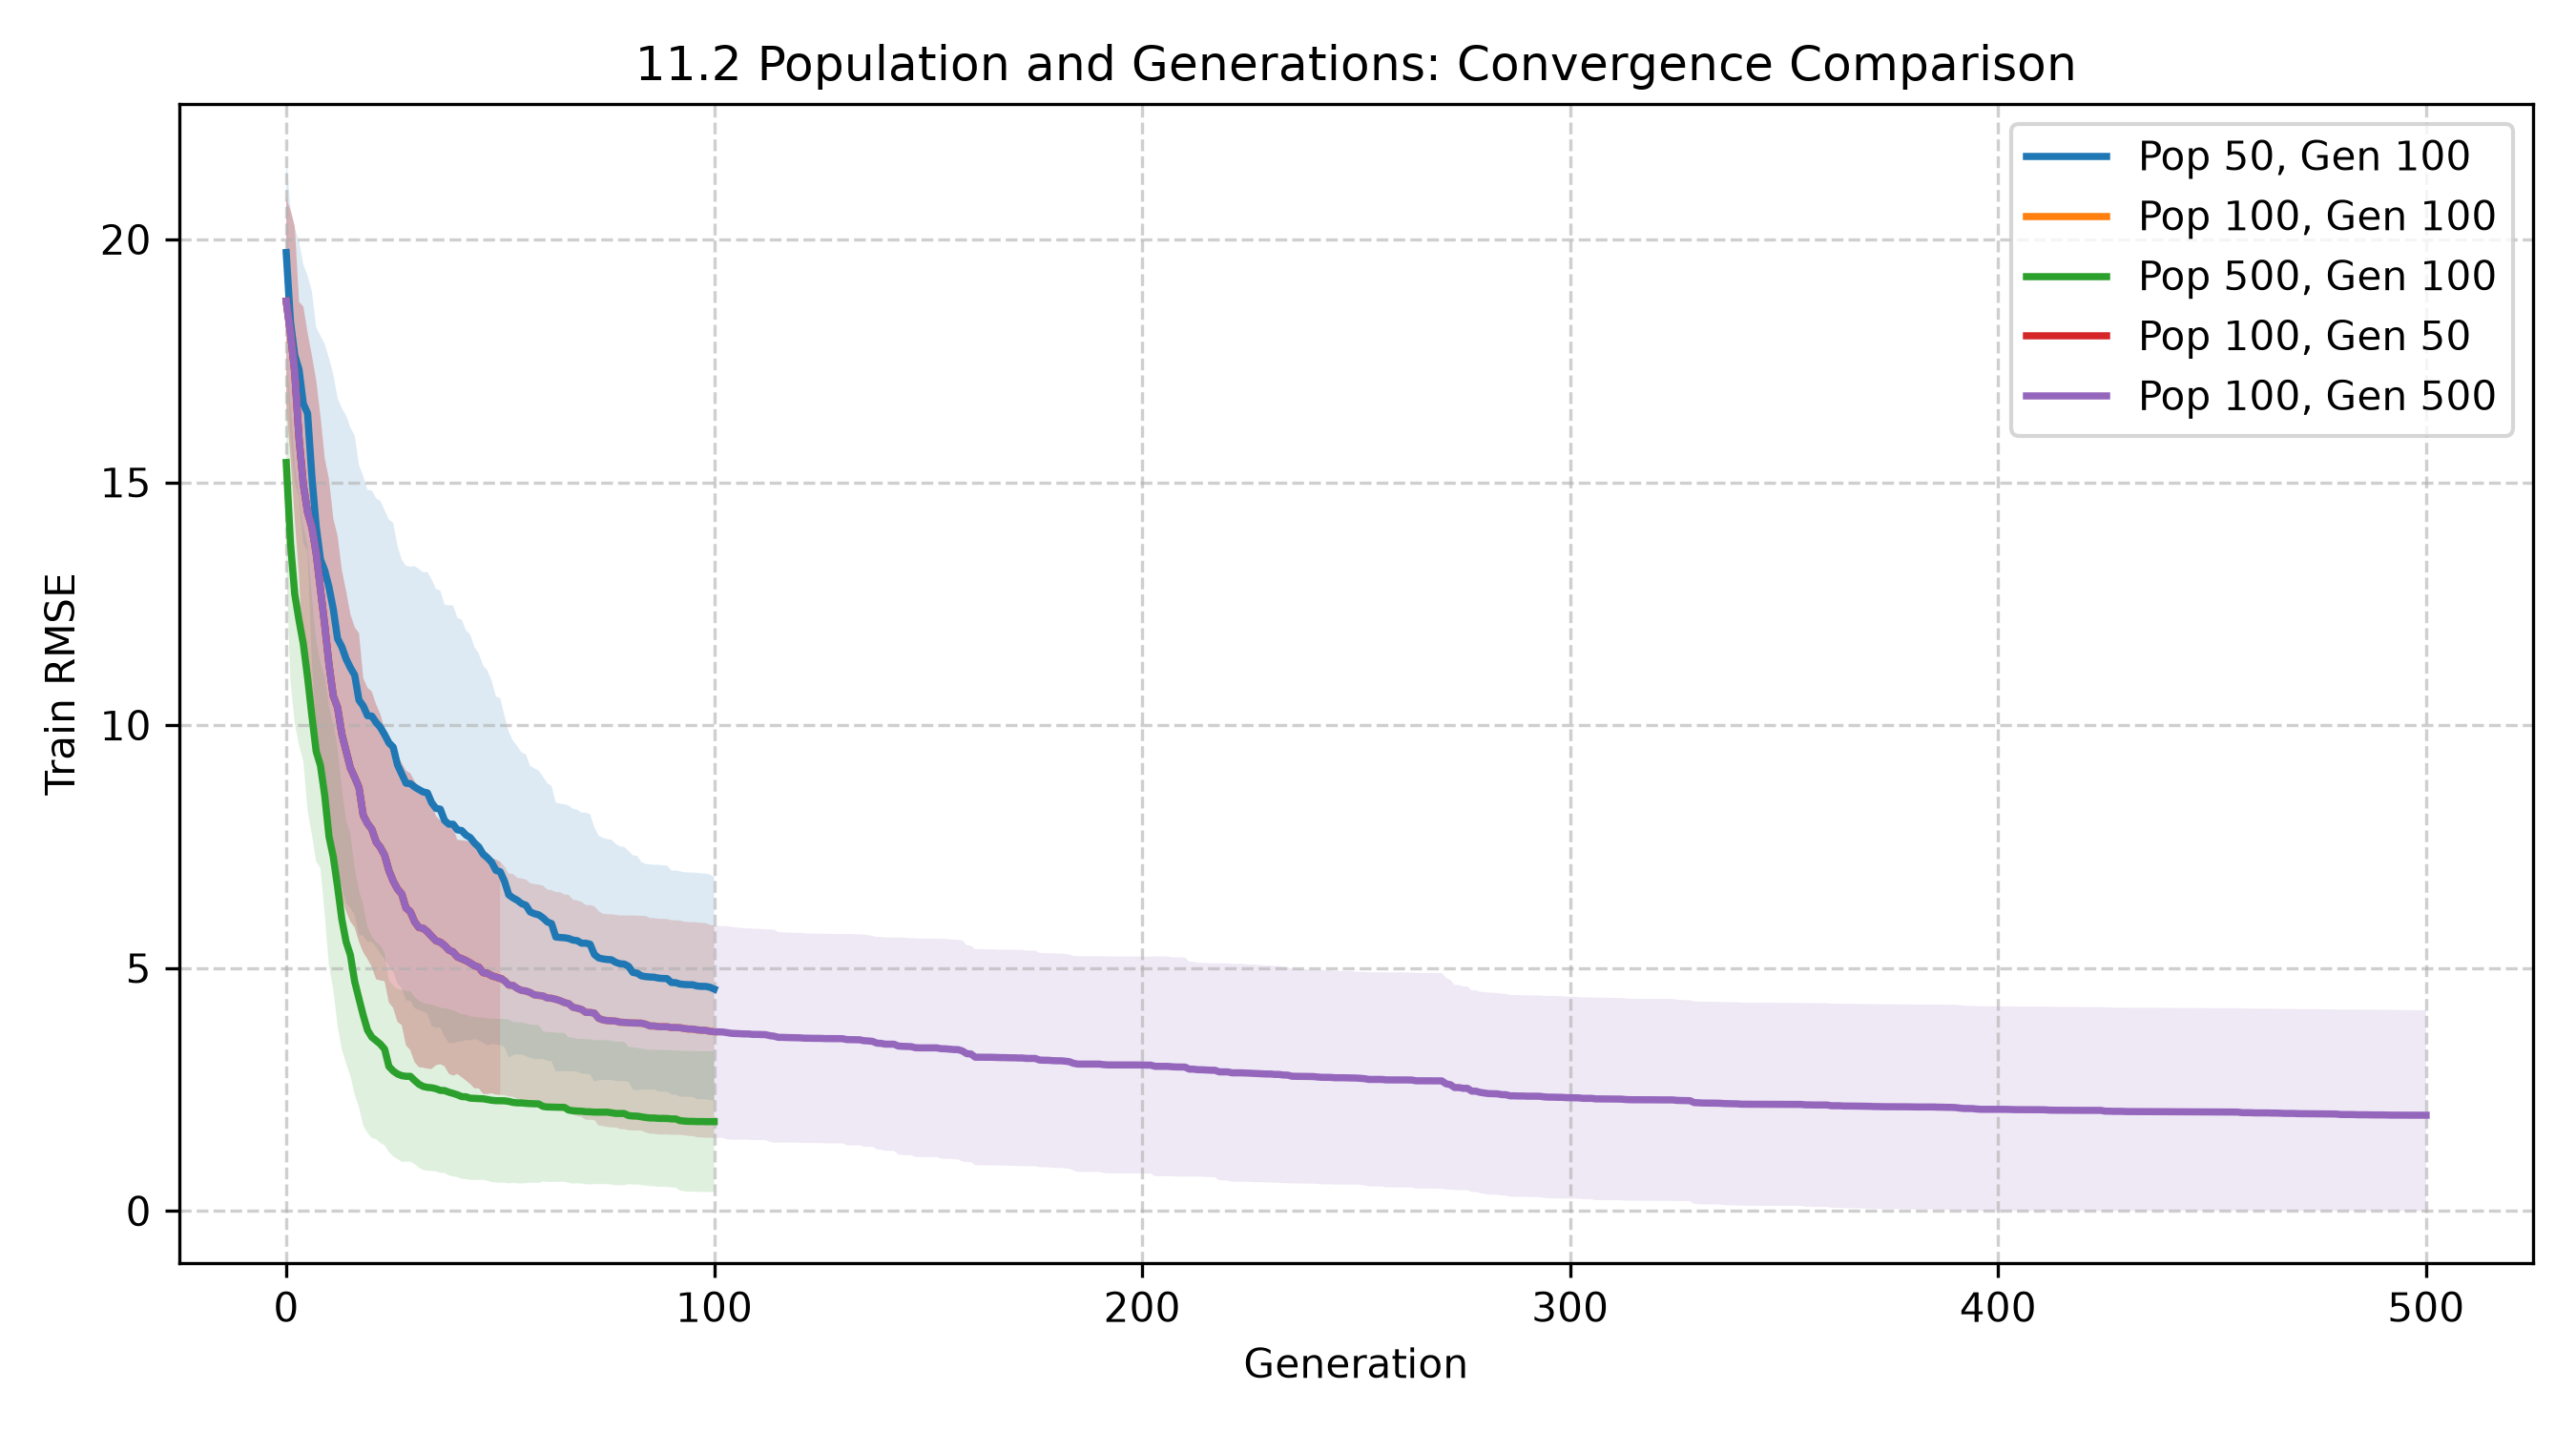
\includegraphics[width=\linewidth]{pop_gens_convergence.png}
    \caption{Convergência (melhor RMSE de treino).}
  \end{subfigure}\hfill
  \begin{subfigure}{0.42\linewidth}
    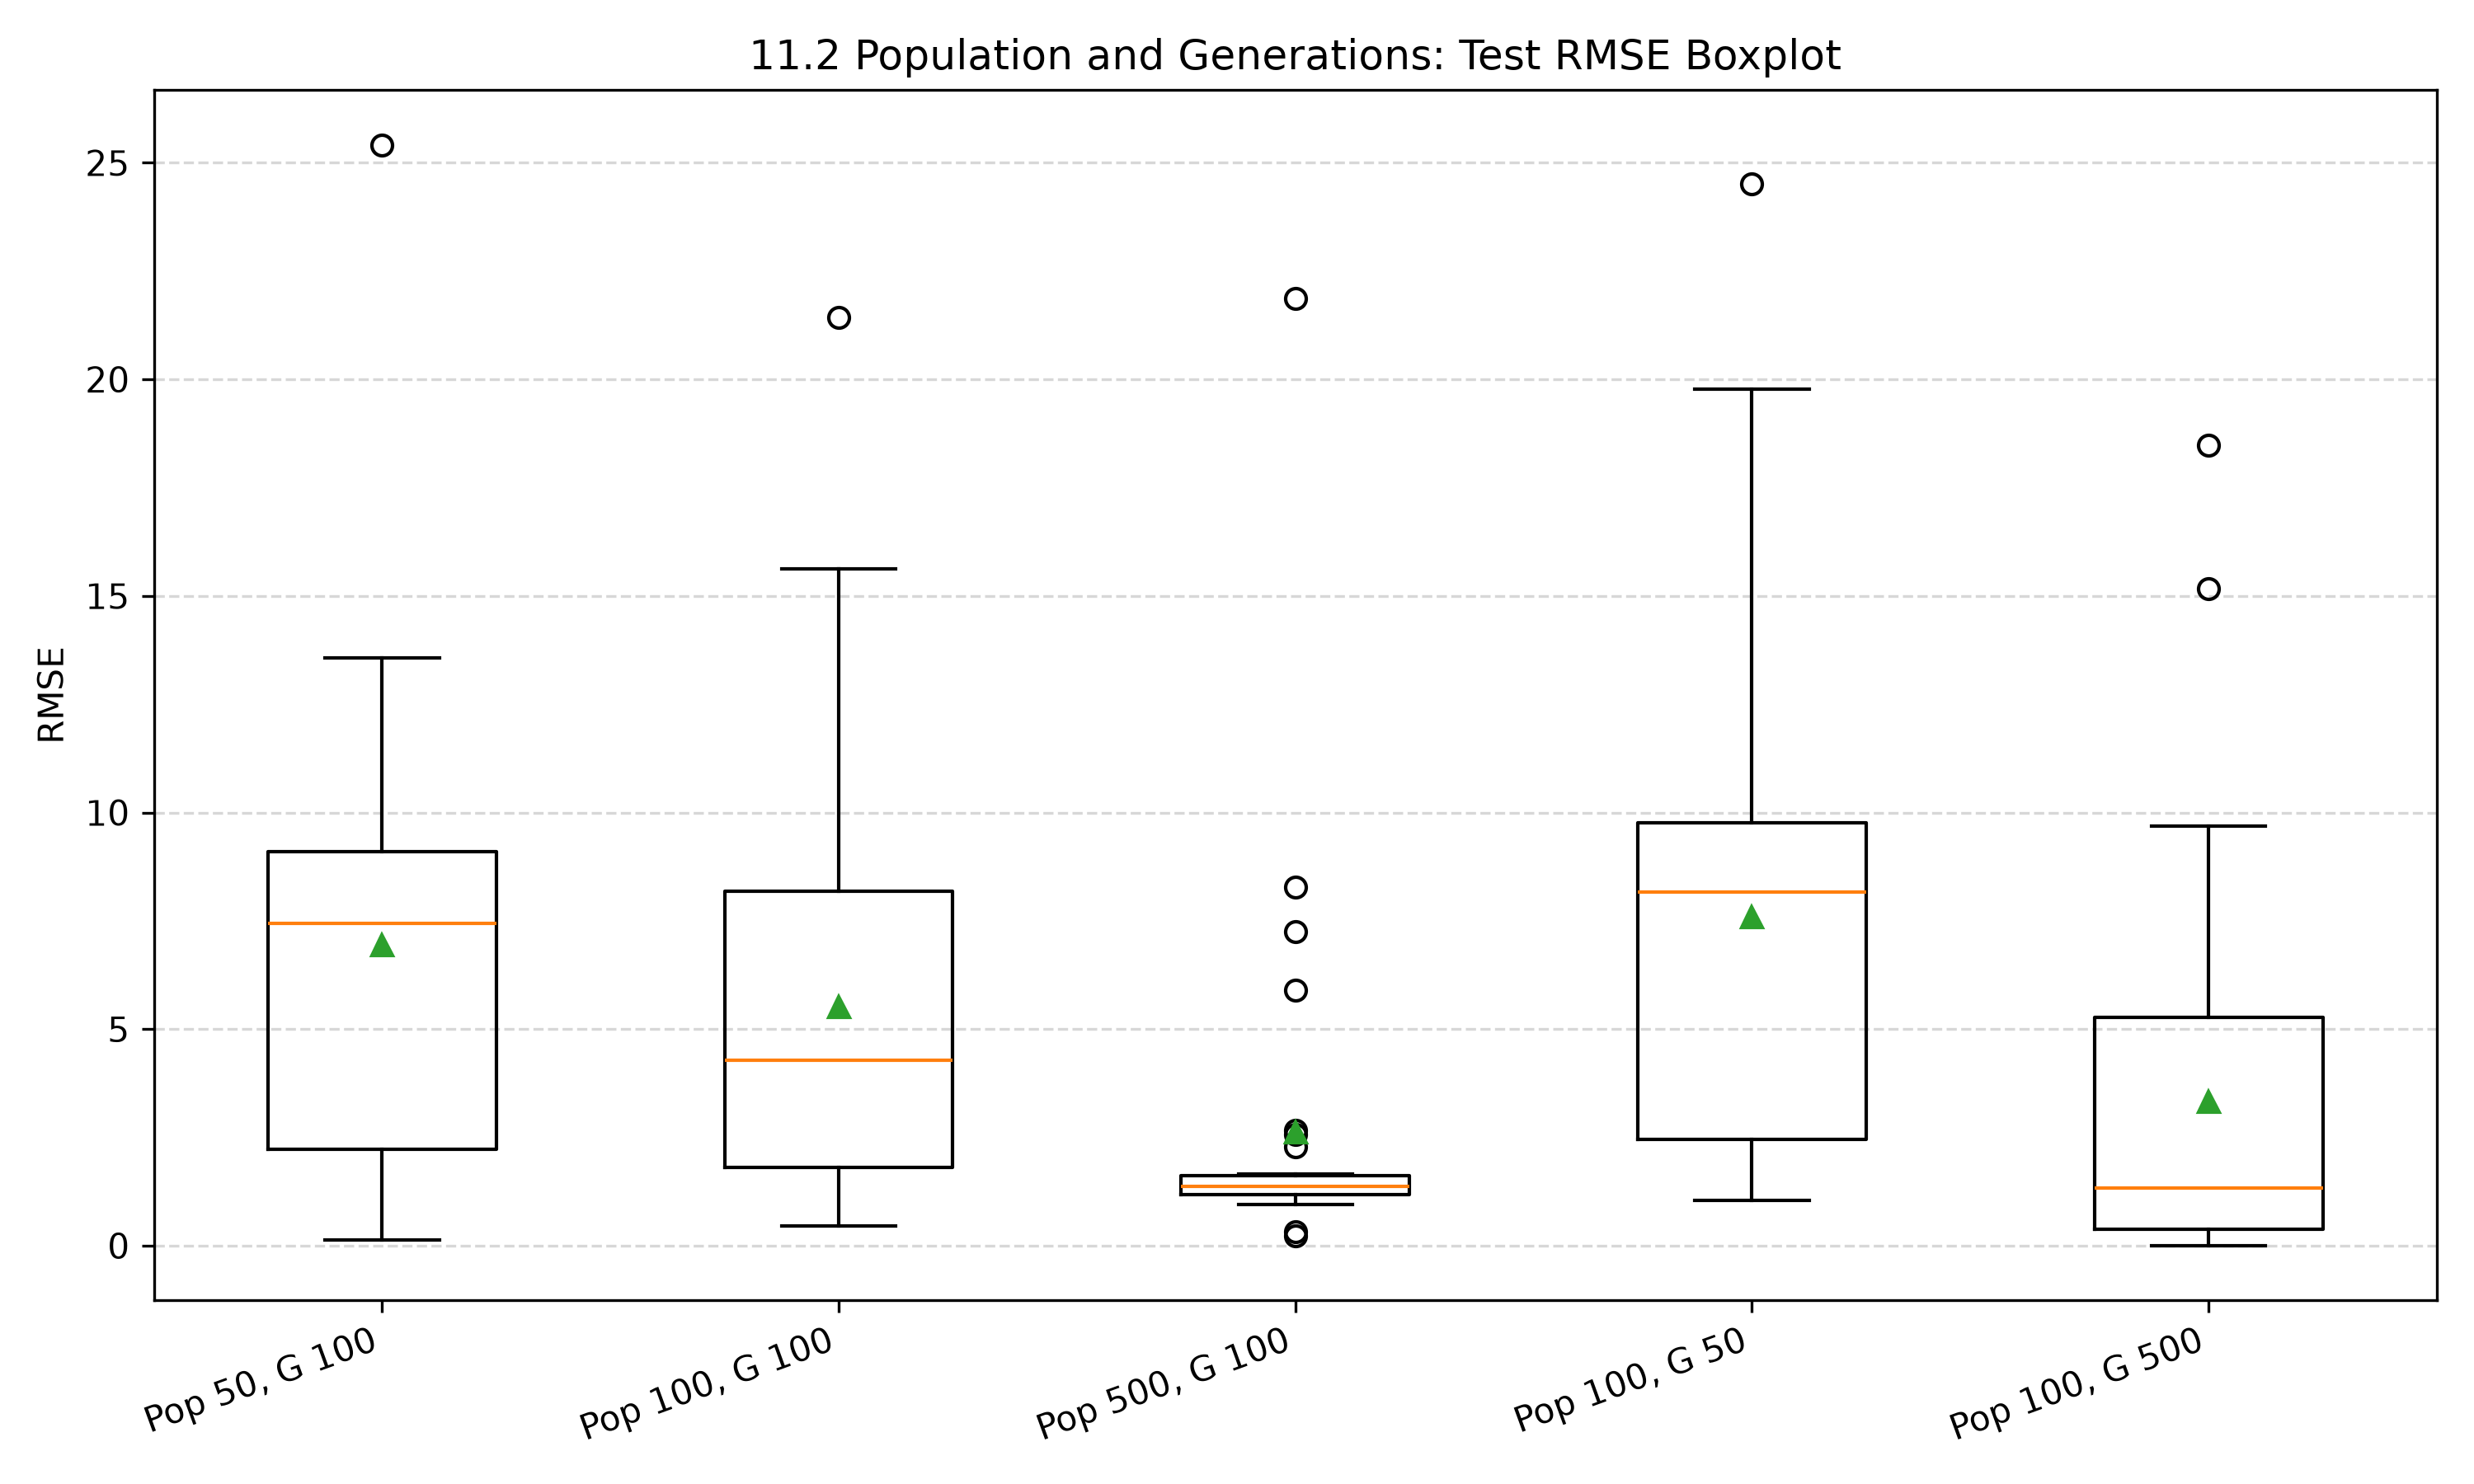
\includegraphics[width=\linewidth]{pop_gens_test_boxplot.png}
    \caption{RMSE de teste.}
  \end{subfigure}
  \caption{Efeito da população e do número de gerações no \code{synth1}.}
  \label{fig:f1_popgen}
\end{figure}

A \cref{tab:f1_popgen} e a \cref{fig:f1_popgen} mostram que aumentar o
orçamento de avaliações reduz o erro: as duas configurações com 50\,000
avaliações são significativamente melhores que a base ($p<0.005$). Já as
configurações com 5\,000 avaliações são piores, embora sem significância a
$5\%$ pelo teste não pareado.

\paragraph{População versus gerações.} Com o mesmo orçamento (50\,000
avaliações), \code{pop=500} e \code{gen=500} não diferem significativamente
na mediana ($p=0.50$), mas \code{pop=500} apresenta IQR dez vezes menor
($0.43$ contra $4.89$), árvores $35\%$ menores ($41.8$ contra $64.2$ nós) e
menor tempo de execução. Prolongar a evolução depois da saturação (por volta
da geração~80) alimenta principalmente o crescimento das árvores, enquanto
ampliar a população aumenta a cobertura do espaço de busca já na geração~0.

\paragraph{A população converge?} Sim. Com 100 gerações, a curva de treino
atinge $95\%$ da melhoria total por volta da geração~80. O número de
indivíduos repetidos atinge um pico na geração~5 (27 de 100 com torneio) e
depois se estabiliza em torno de 9--11, indicando perda parcial de
diversidade.

\paragraph{Escolha.} Foi mantido \code{pop=100}, \code{gen=100}: é a menor
configuração que satura dentro do orçamento, e é cerca de $6\times$ mais
barata que \code{pop=500}, o que viabilizou as mais de 1\,900 execuções do
estudo. Reconhece-se, porém, que \code{pop=500} seria preferível se o custo
não fosse restritivo.

% -----------------------------------------------------------------------------
\subsubsection{Métodos de seleção}
\label{sec:f1_selecao}

\begin{table}[htbp]
  \centering
  \caption{Métodos de seleção no \code{synth1}. ``Rep.'' é o número médio de
           indivíduos repetidos nas gerações 0, 5, 20 e final. Valores de $p$
           (Mann--Whitney) em relação ao torneio com $k=2$.}
  \label{tab:f1_selecao}
  \small
  \resizebox{\linewidth}{!}{%
  \begin{tabular}{@{}lcccccccr@{}}
    \toprule
    Seleção & RMSE treino & RMSE teste & Mediana (IQR) & Mín./Máx. & $p$ & Sat. & Rep. (G0/5/20/F) & Tempo (s) \\
    \midrule
    Roleta          & $3.16 \pm 2.24$ & $5.66 \pm 8.85$  & 2.17 (7.28) & 0.70 / 48.36  & 0.595 & 80 & 10.5/20.3/14.5/9.1 & 7.8 \\
    Torneio $k=2$   & $3.69 \pm 2.19$ & $5.52 \pm 4.89$  & 4.28 (6.38) & 0.46 / 21.44  & ---   & 80 & 10.5/27.1/10.8/9.0 & 7.8 \\
    Torneio $k=3$   & $4.06 \pm 2.20$ & $13.33 \pm 42.80$& 7.01 (6.38) & 0.20 / 239.17 & 0.530 & 63 & 10.5/26.1/14.0/13.9 & 6.6 \\
    \rowcolor{verde}
    $\eps$-Lexicase & $\mathbf{0.99 \pm 1.21}$ & $\mathbf{1.62 \pm 3.36}$ & \textbf{0.68 (1.12)} & 0.01 / 18.19 & $\mathbf{4.1{\times}10^{-6}}$ & 94 & 10.5/\textbf{4.0}/8.7/13.4 & 22.5 \\
    \bottomrule
  \end{tabular}}
\end{table}

\begin{figure}[htbp]
  \centering
  \begin{subfigure}{0.49\linewidth}
    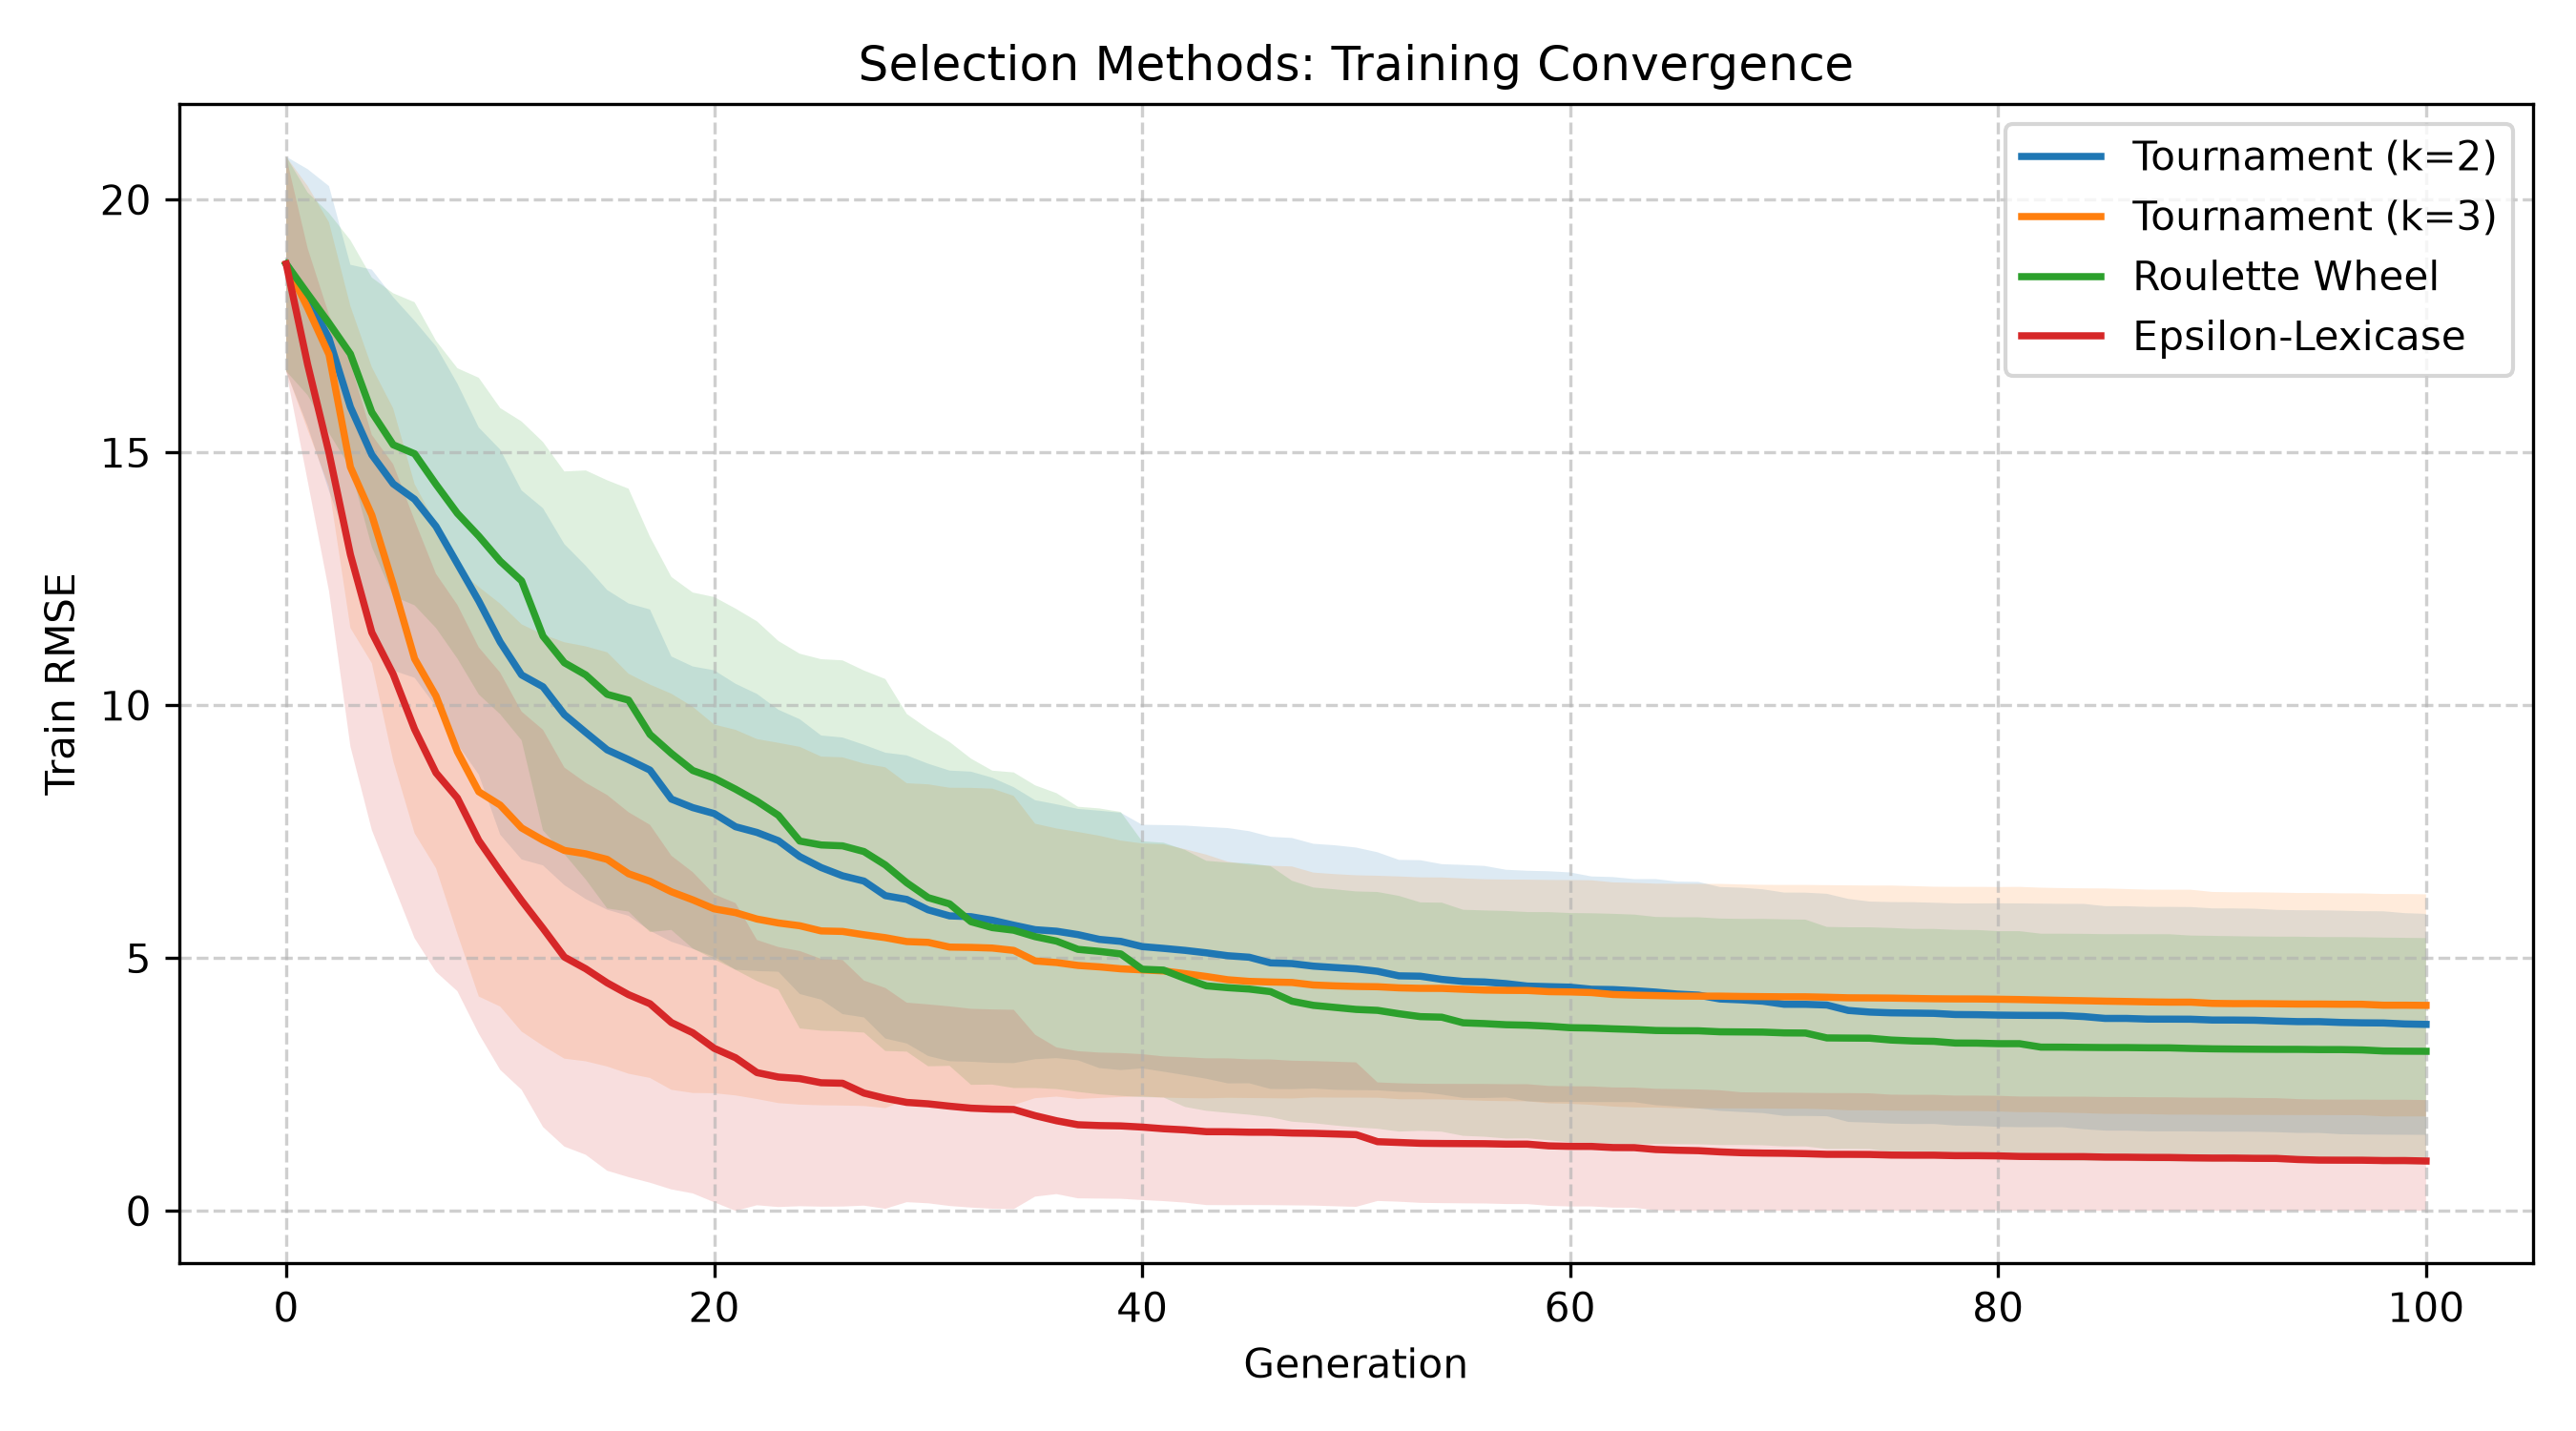
\includegraphics[width=\linewidth]{selection_convergence.png}
    \caption{Convergência.}
  \end{subfigure}\hfill
  \begin{subfigure}{0.49\linewidth}
    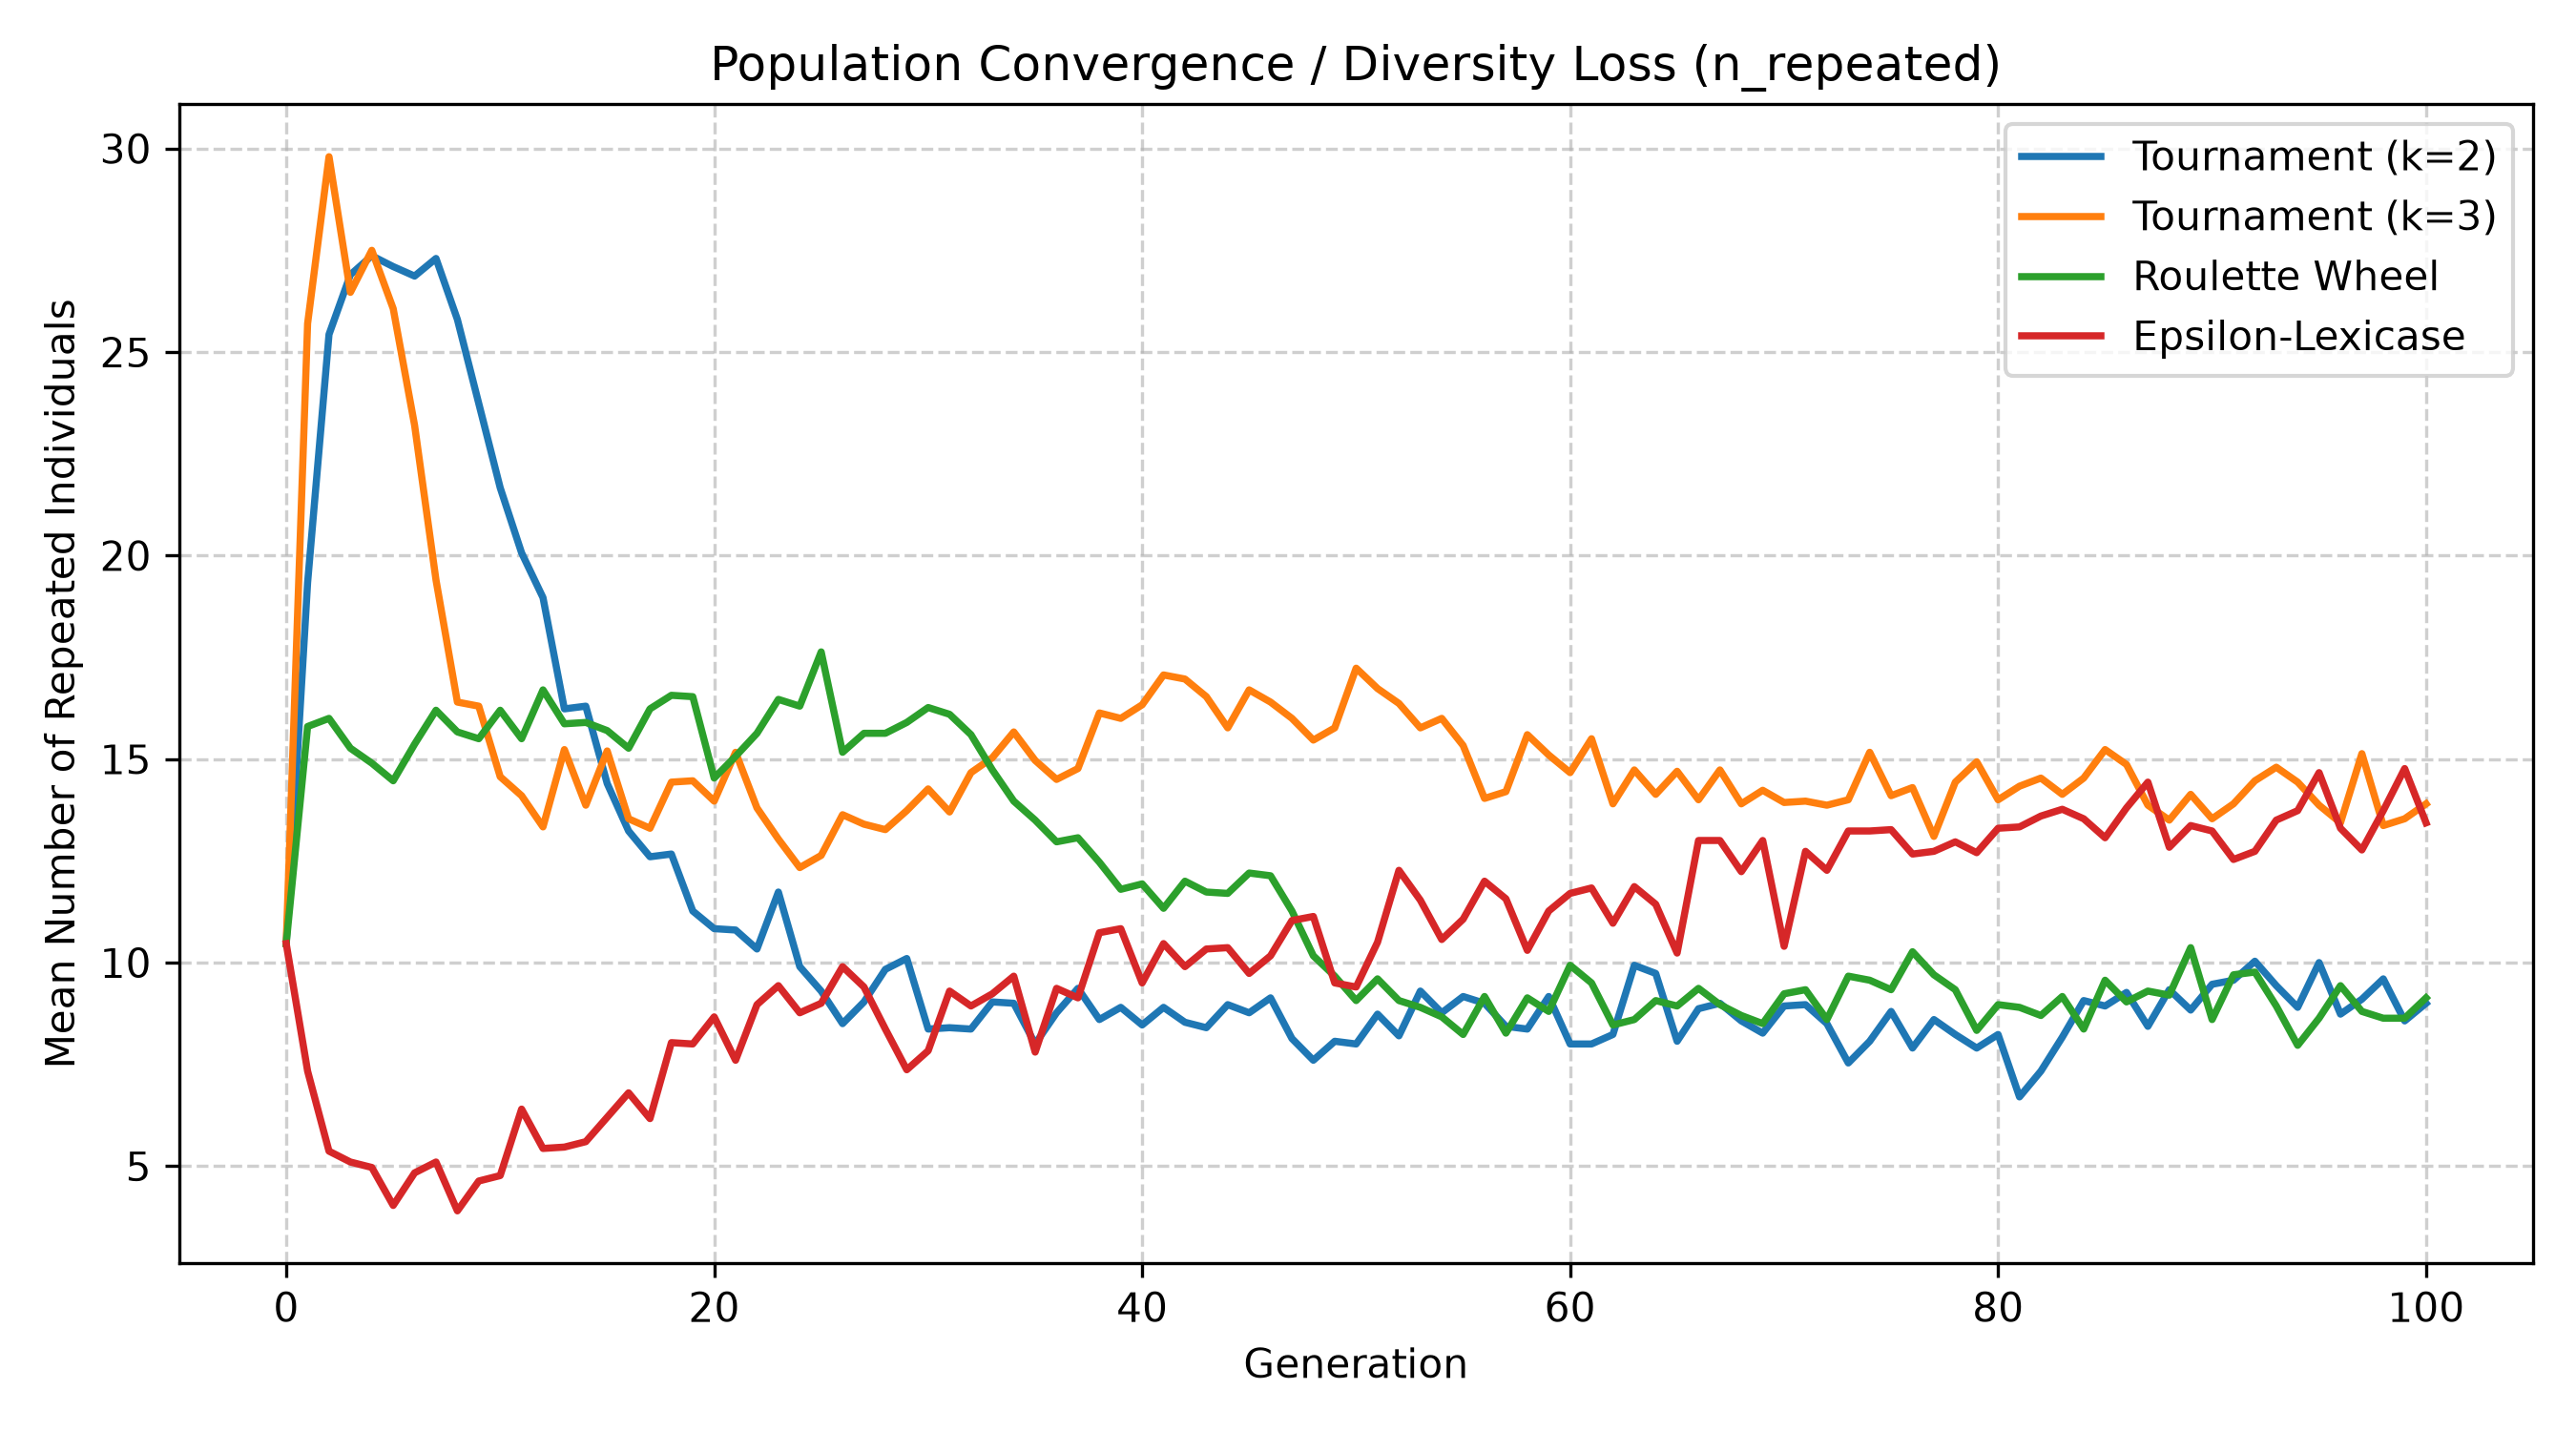
\includegraphics[width=\linewidth]{selection_diversity_n_repeated.png}
    \caption{Indivíduos repetidos por geração.}
  \end{subfigure}
  \caption{Dinâmica dos métodos de seleção no \code{synth1}.}
  \label{fig:f1_selecao}
\end{figure}

A $\eps$-lexicase foi o \textbf{único fator da Fase~1 com efeito
estatisticamente significativo} sobre a configuração base
(\cref{tab:f1_selecao}): o RMSE médio de teste caiu $70.7\%$
($5.52\to1.62$; $p=4.1\times10^{-6}$; 26 vitórias em 30 sementes), e a mediana
caiu de $4.28$ para $0.68$. As mudanças observadas ao trocar a seleção foram:

\begin{itemize}
  \item \textbf{Roleta:} a transformação $1/(1+\mathrm{RMSE})$ achata as
        diferenças entre indivíduos e reduz a pressão seletiva. O resultado
        não difere significativamente do torneio ($p=0.595$), mas a
        variância no teste é muito maior (desvio de $8.85$, máximo de
        $48.4$).
  \item \textbf{Torneio $k=3$:} o aumento da pressão seletiva antecipa a
        saturação (geração~63 contra~80) e produz execuções catastróficas no
        teste (máximo de $239$), um sinal de convergência prematura para
        expressões que extrapolam mal.
  \item \textbf{$\eps$-Lexicase:} na geração~5, o número de clones cai de
        27.1 (torneio) para 4.0, e a população continua melhorando até a
        geração~94 (\cref{fig:f1_selecao}). Ao selecionar especialistas em
        subconjuntos distintos de casos, o método mantém múltiplas
        linhagens e evita que um único indivíduo domine a população cedo.
        O custo é cerca de $3\times$ maior, devido à filtragem caso a caso.
\end{itemize}

% -----------------------------------------------------------------------------
\subsubsection{\emph{Crossover} e mutação}
\label{sec:f1_operadores}

Conforme estabelecido no guia experimental do enunciado, foram investigadas duas
configurações de partida para os operadores genéticos de variação:
(i)~\textbf{Configuração~A} ($\pc=0.90$, $\pmut=0.05$), que adota o regime
canônico clássico de Koza onde o \emph{crossover} atua como o principal motor
evolutivo e a mutação é mantida em nível residual; e
(ii)~\textbf{Configuração~B} ($\pc=0.60$, $\pmut=0.30$), que testa uma hipótese
balanceada com mutação substancialmente mais agressiva ($6\times$ superior) e
cruzamento atenuado, investigando se uma exploração local mais frequente previne
a estagnação prematura. Subsequentemente, realizaram-se varreduras
unidimensionais de $\pc\in\{0.5,0.7,0.9\}$ e $\pmut\in\{0.01,0.05,0.1,0.2\}$,
todas fixando seleção por torneio $k=2$ (\cref{tab:f1_operadores}).

\begin{table}[htbp]
  \centering
  \caption{Contribuição dos operadores no \code{synth1} (totais médios por
           execução em 100 gerações). ``Cx $>$ média'' e ``Cx $>$ melhor''
           indicam a fração de filhos de \emph{crossover} melhores que a
           média dos pais e que o melhor pai, respectivamente.}
  \label{tab:f1_operadores}
  \small
  \resizebox{\linewidth}{!}{%
  \begin{tabular}{@{}lccccccc@{}}
    \toprule
    Config. & Cx melhor/pior (média pais) & Cx $>$ média & Cx $>$ melhor & Mut. $+$ (bruta)$^a$ & Mut. $+$ (corrigida)$^b$ & RMSE teste & Mediana (IQR) \\
    \midrule
    A: $\pc{=}0.9$, $\pmut{=}0.05$ & 2643.6 / 5606.1 & 32.0\% & 11.0\% & 92.5\% & $\approx$25\% & $5.52 \pm 4.89$ & 4.28 (6.38) \\
    B: $\pc{=}0.6$, $\pmut{=}0.30$ & 1233.5 / 2894.4 & 29.9\% & 11.5\% & 69.3\% & $\approx$23\% & $5.96 \pm 4.52$ & 7.79 (7.98) \\
    \midrule
    $\pc{=}0.5$, $\pmut{=}0.05$    &  955.6 / 3516.4 & 21.4\% &  5.4\% & 56.4\% & $\approx$13\% & $7.92 \pm 9.12$ & 7.48 (7.16) \\
    \rowcolor{verde}
    $\pc{=}0.7$, $\pmut{=}0.05$    & 1744.5 / 4627.2 & 27.4\% &  8.5\% & 75.9\% & $\approx$20\% & $3.97 \pm 3.41$ & 2.09 (6.54) \\
    $\pc{=}0.9$, $\pmut{=}0.01$    & 2709.6 / 5886.8 & 31.5\% & 10.5\% & 92.5\% & $\approx$25\% & $6.46 \pm 4.27$ & 7.26 (6.26) \\
    \rowcolor{verde}
    $\pc{=}0.9$, $\pmut{=}0.10$    & 2575.9 / 5332.8 & 32.6\% & 12.3\% & 92.2\% & $\approx$22\% & $3.89 \pm 3.15$ & 2.47 (5.93) \\
    $\pc{=}0.9$, $\pmut{=}0.20$    & 2390.5 / 4693.7 & 33.7\% & 13.9\% & 92.8\% & $\approx$28\% & $6.53 \pm 4.16$ & 8.03 (6.70) \\
    \bottomrule
  \end{tabular}}

  \vspace{3pt}
  \raggedright\footnotesize
  $^a$ Fração de mutações que melhoraram a aptidão, conforme registrada pelo arcabouço.\\
  $^b$ Estimativa que remove o artefato descrito no texto: $(b-\pc N)/((1-\pc)N)$, com $b$ o número de mutações benéficas e $N$ o total de mutações não neutras.
\end{table}

\begin{figure}[htbp]
  \centering
  \begin{subfigure}{0.49\linewidth}
    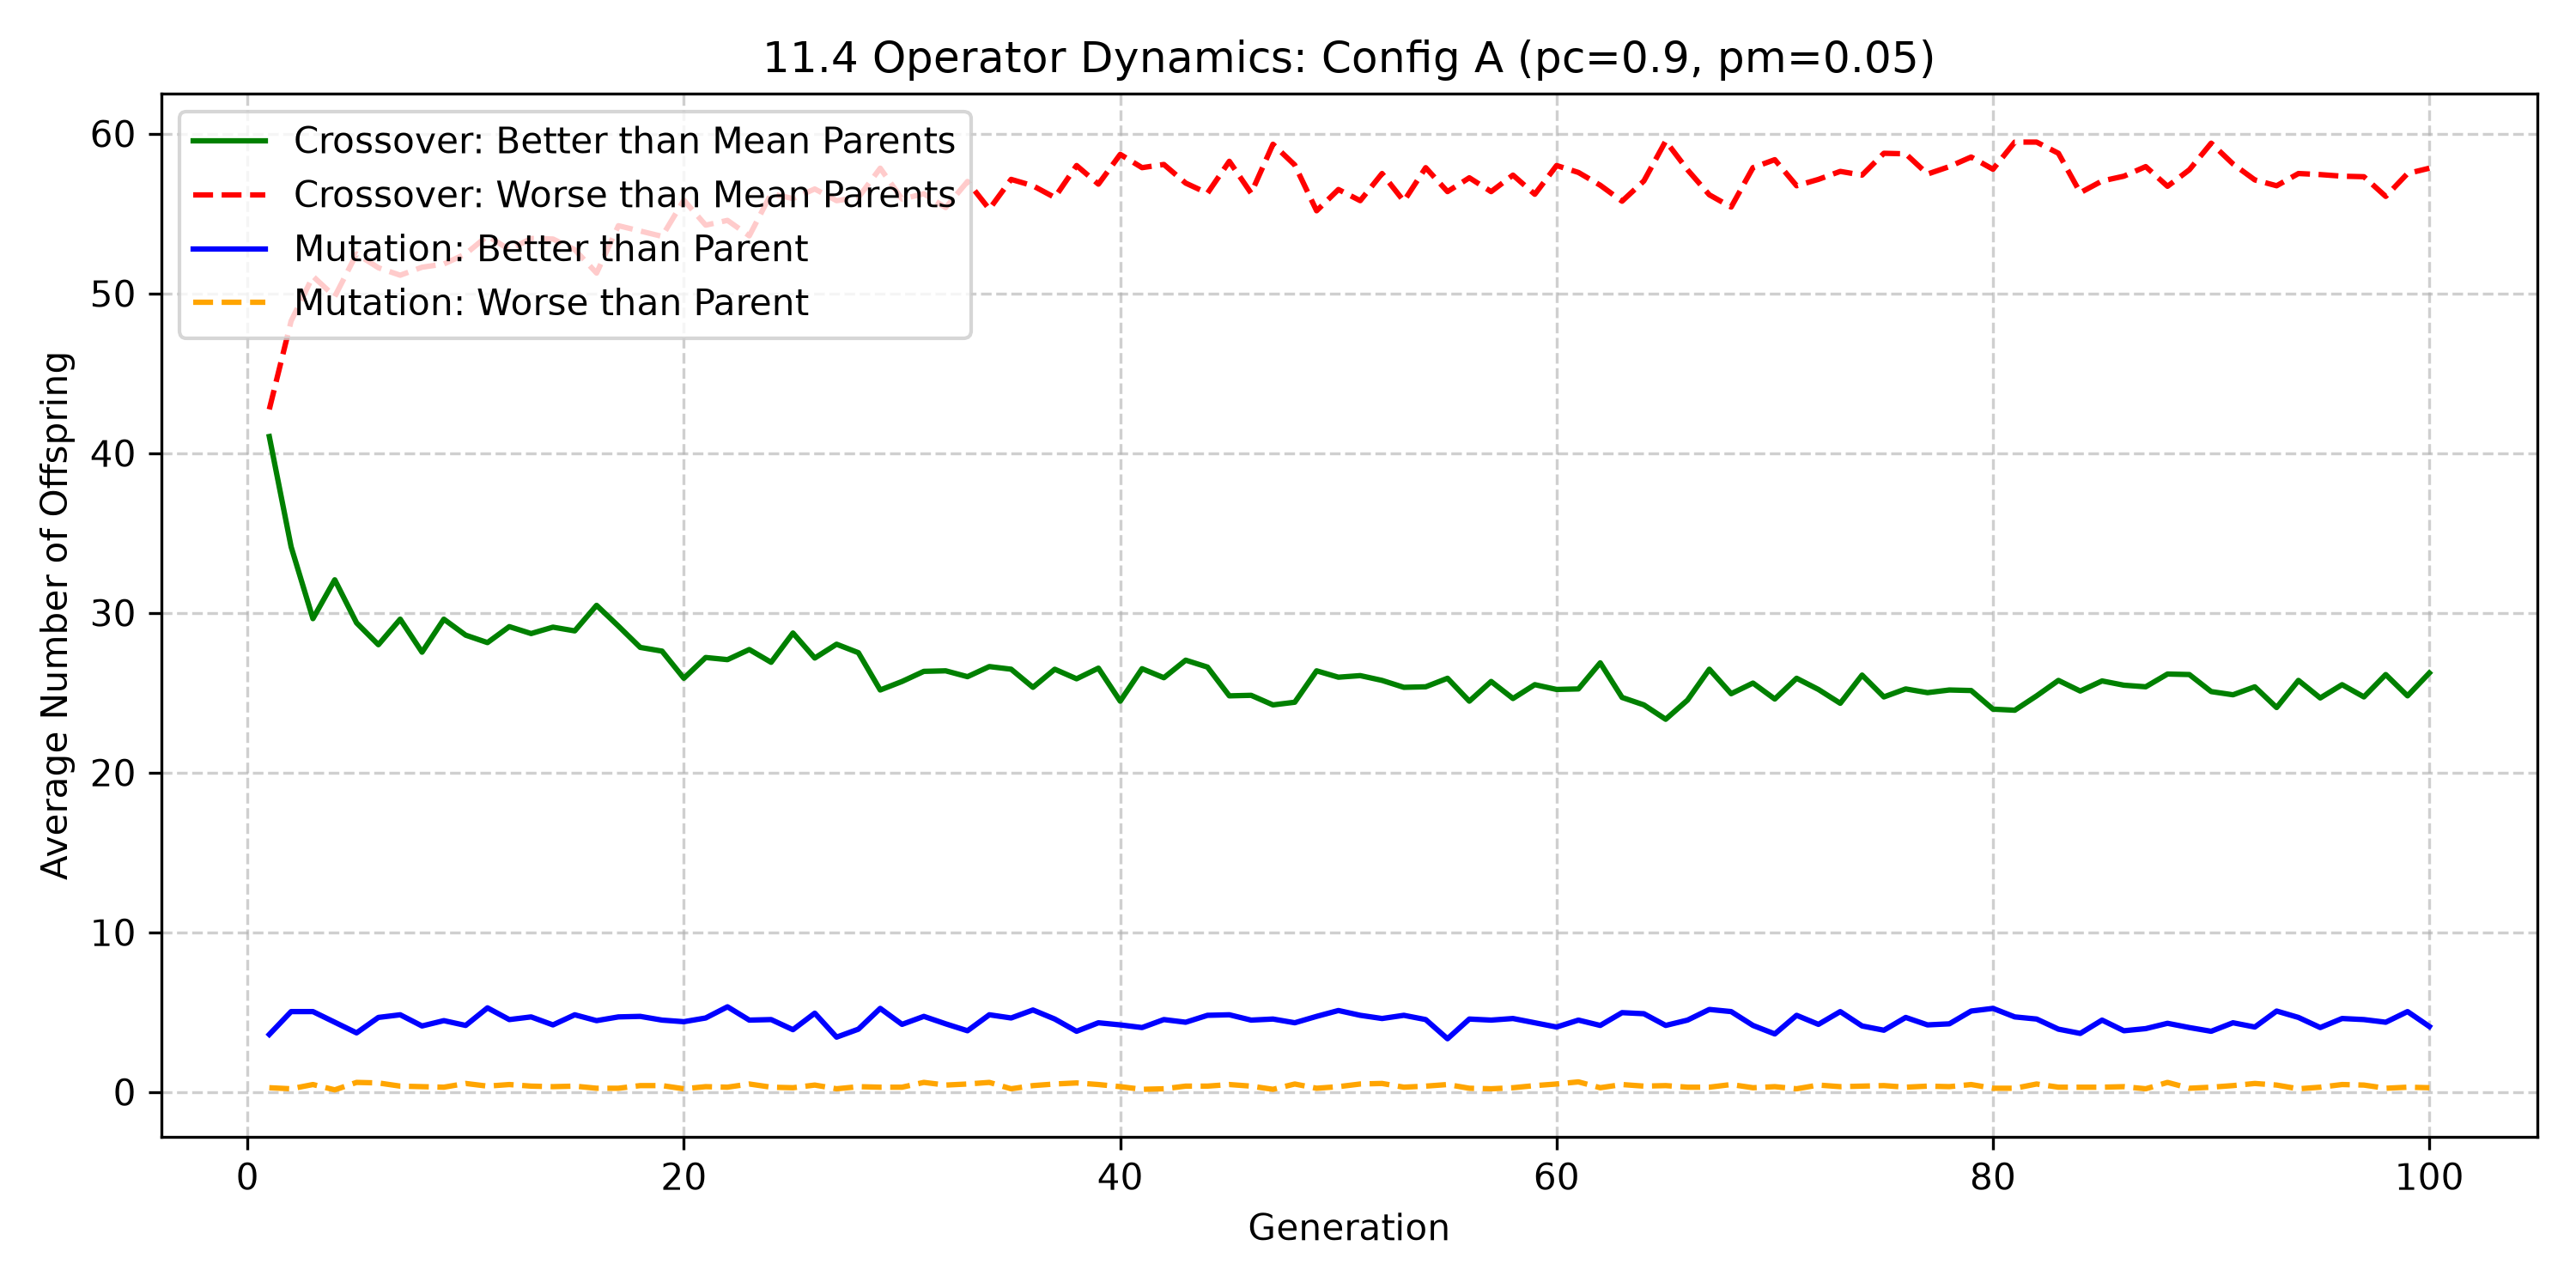
\includegraphics[width=\linewidth]{operator_dynamics_config_A.png}
    \caption{Config.~A ($\pc=0.9$, $\pmut=0.05$).}
  \end{subfigure}\hfill
  \begin{subfigure}{0.49\linewidth}
    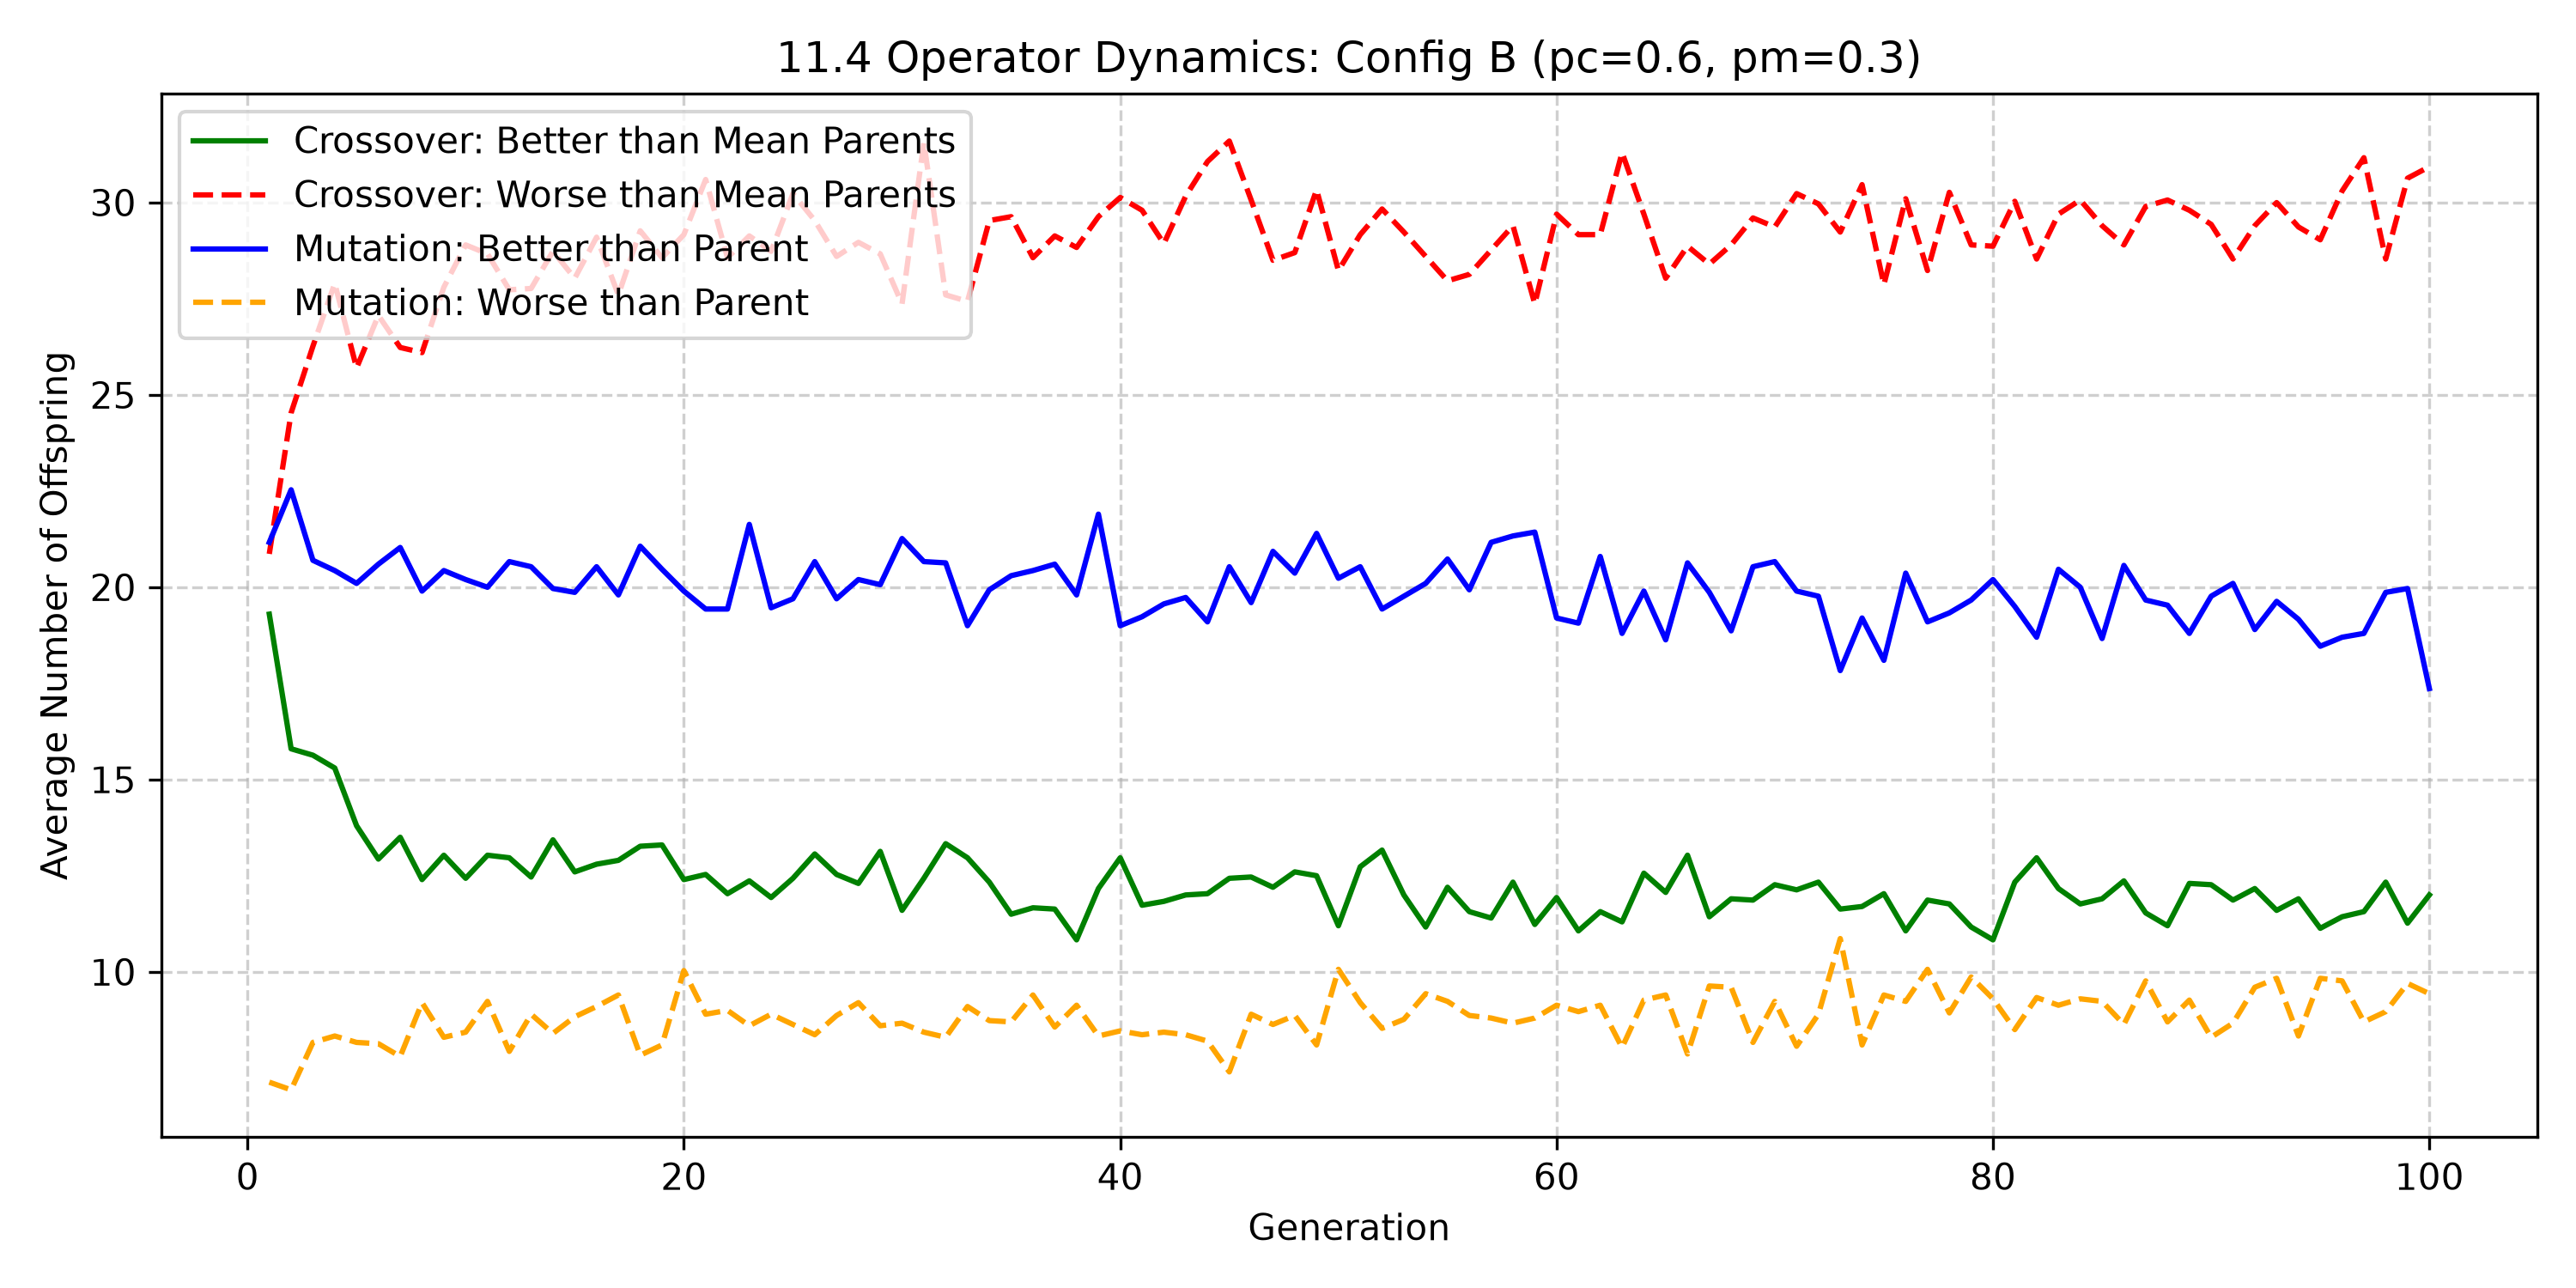
\includegraphics[width=\linewidth]{operator_dynamics_config_B.png}
    \caption{Config.~B ($\pc=0.6$, $\pmut=0.3$).}
  \end{subfigure}
  \caption{Número de filhos melhores e piores que os pais por geração.}
  \label{fig:f1_operadores}
\end{figure}

\paragraph{Em quantos casos cada operador contribui?} O \emph{crossover} é
predominantemente destrutivo: na Config.~A, apenas $32\%$ dos filhos superam
a média dos pais e apenas $11\%$ superam o melhor pai, ou seja, $89\%$ das
recombinações pioram o melhor material genético disponível. A
\cref{fig:f1_operadores} mostra que a fração positiva é máxima nas primeiras
gerações (cerca de 41 filhos melhores que a média dos pais na geração~1) e
cai rapidamente para cerca de 25 por geração, à medida que a população se
especializa e a troca de subárvores passa a desmontar expressões já
ajustadas. A produtividade em relação ao melhor pai cai de $10.1$ filhos por
geração (gerações 1--20) para $6.8$ (gerações 81--100).

\paragraph{Artefato na métrica de mutação.} A taxa de sucesso bruta da
mutação ($\approx92\%$ com $\pc=0.9$) está \textbf{superestimada}. Quando a
mutação é aplicada a um filho recém-gerado por \emph{crossover}, esse filho
ainda não foi avaliado, e a sua aptidão ``anterior'' é registrada como
$+\infty$. Assim, toda mutação pós-\emph{crossover} é contada como benéfica.
O indício é que a taxa bruta acompanha $\pc$ (56\%, 69\%, 76\% e 92\% para
$\pc=0.5$, $0.6$, $0.7$ e $0.9$). Removendo a fração esperada de casos
contaminados, a taxa real de mutações benéficas fica entre $13\%$ e $28\%$
(\cref{tab:f1_operadores}). Ou seja, a mutação de subárvore também é
majoritariamente destrutiva, embora menos que o \emph{crossover} em relação
ao melhor pai. O artefato não afeta a evolução, apenas a estatística.

\paragraph{Config.~A versus Config.~B.} Não há diferença significativa
($p=0.641$). A Config.~B produz árvores menores ($37.5$ contra $46.5$ nós),
mas a mutação de subárvore a $30\%$ substitui blocos inteiros de soluções
boas, e a mediana sobe de $4.28$ para $7.79$.

\paragraph{Valores propostos.} As varreduras indicam um ótimo
\emph{intermediário}: tanto reduzir $\pc$ para $0.7$ (mediana $2.09$) quanto
elevar $\pmut$ para $0.1$ (mediana $2.47$) melhoram a configuração base, e os
extremos ($\pc=0.5$, $\pmut=0.01$ ou $\pmut=0.2$) pioram. Nenhuma dessas
diferenças é significativa isoladamente ($p>0.3$), por causa da
bimodalidade. A proposta resultante, $\pc\approx0.7$ e
$\pmut\in[0.1,0.15]$, \textbf{não foi testada em conjunto na Fase~1}, mas ela foi
validada na Fase~2 (hipótese H2). Os parâmetros anteriores (população e
gerações) permanecem adequados: em todas as varreduras, a saturação ocorre
antes da geração~100.

% -----------------------------------------------------------------------------
\subsubsection{Elitismo}
\label{sec:f1_elitismo}

\begin{table}[htbp]
  \centering
  \caption{Efeito do elitismo no \code{synth1} (torneio $k=2$).}
  \label{tab:f1_elitismo}
  \small
  \begin{tabular}{@{}lccccc@{}}
    \toprule
    Configuração & RMSE treino & RMSE teste & Mediana (IQR) & Mín./Máx. & Tam. melhor \\
    \midrule
    \rowcolor{verde}
    Com elitismo (1) & $3.69 \pm 2.19$ & $5.52 \pm 4.89$ & 4.28 (6.38) & 0.46 / 21.44 & $46.5 \pm 17.5$ \\
    Sem elitismo     & $4.91 \pm 1.91$ & $6.57 \pm 3.07$ & 8.16 (2.90) & 0.94 / 10.97 & $54.3 \pm 15.6$ \\
    \bottomrule
  \end{tabular}
\end{table}

\begin{figure}[htbp]
  \centering
  \begin{subfigure}{0.56\linewidth}
    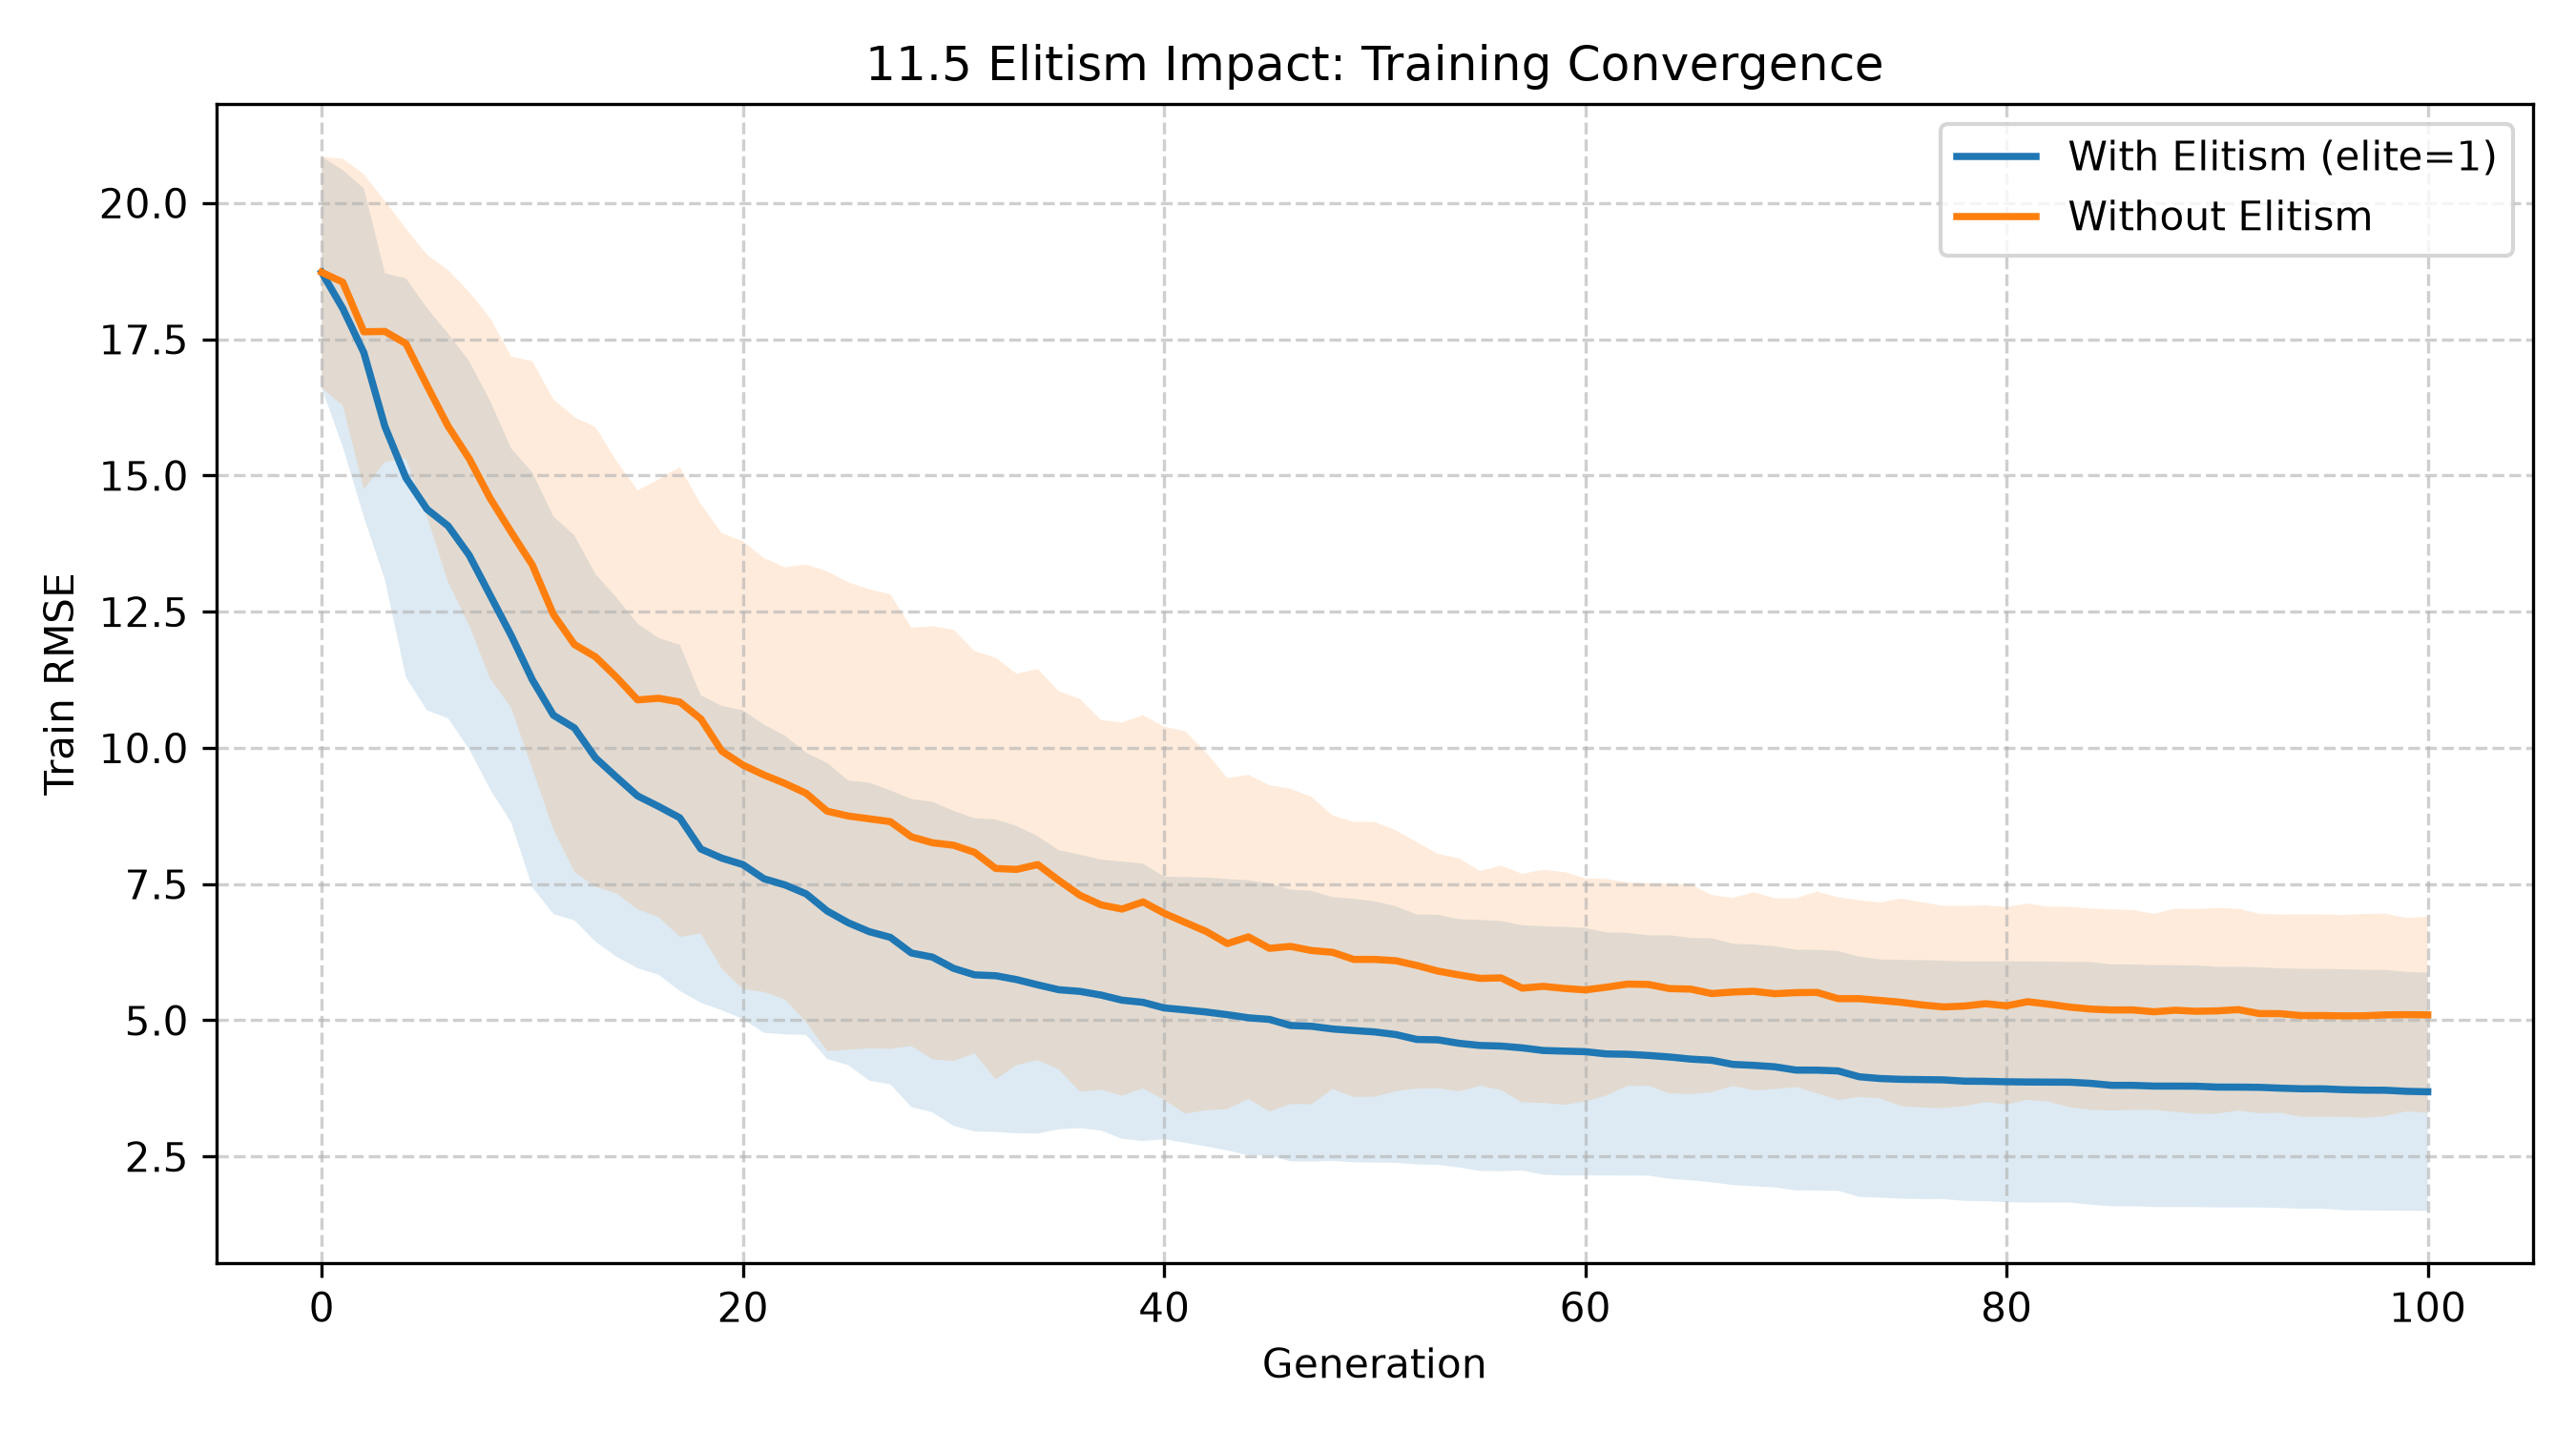
\includegraphics[width=\linewidth]{elitism_convergence.png}
  \end{subfigure}\hfill
  \begin{subfigure}{0.42\linewidth}
    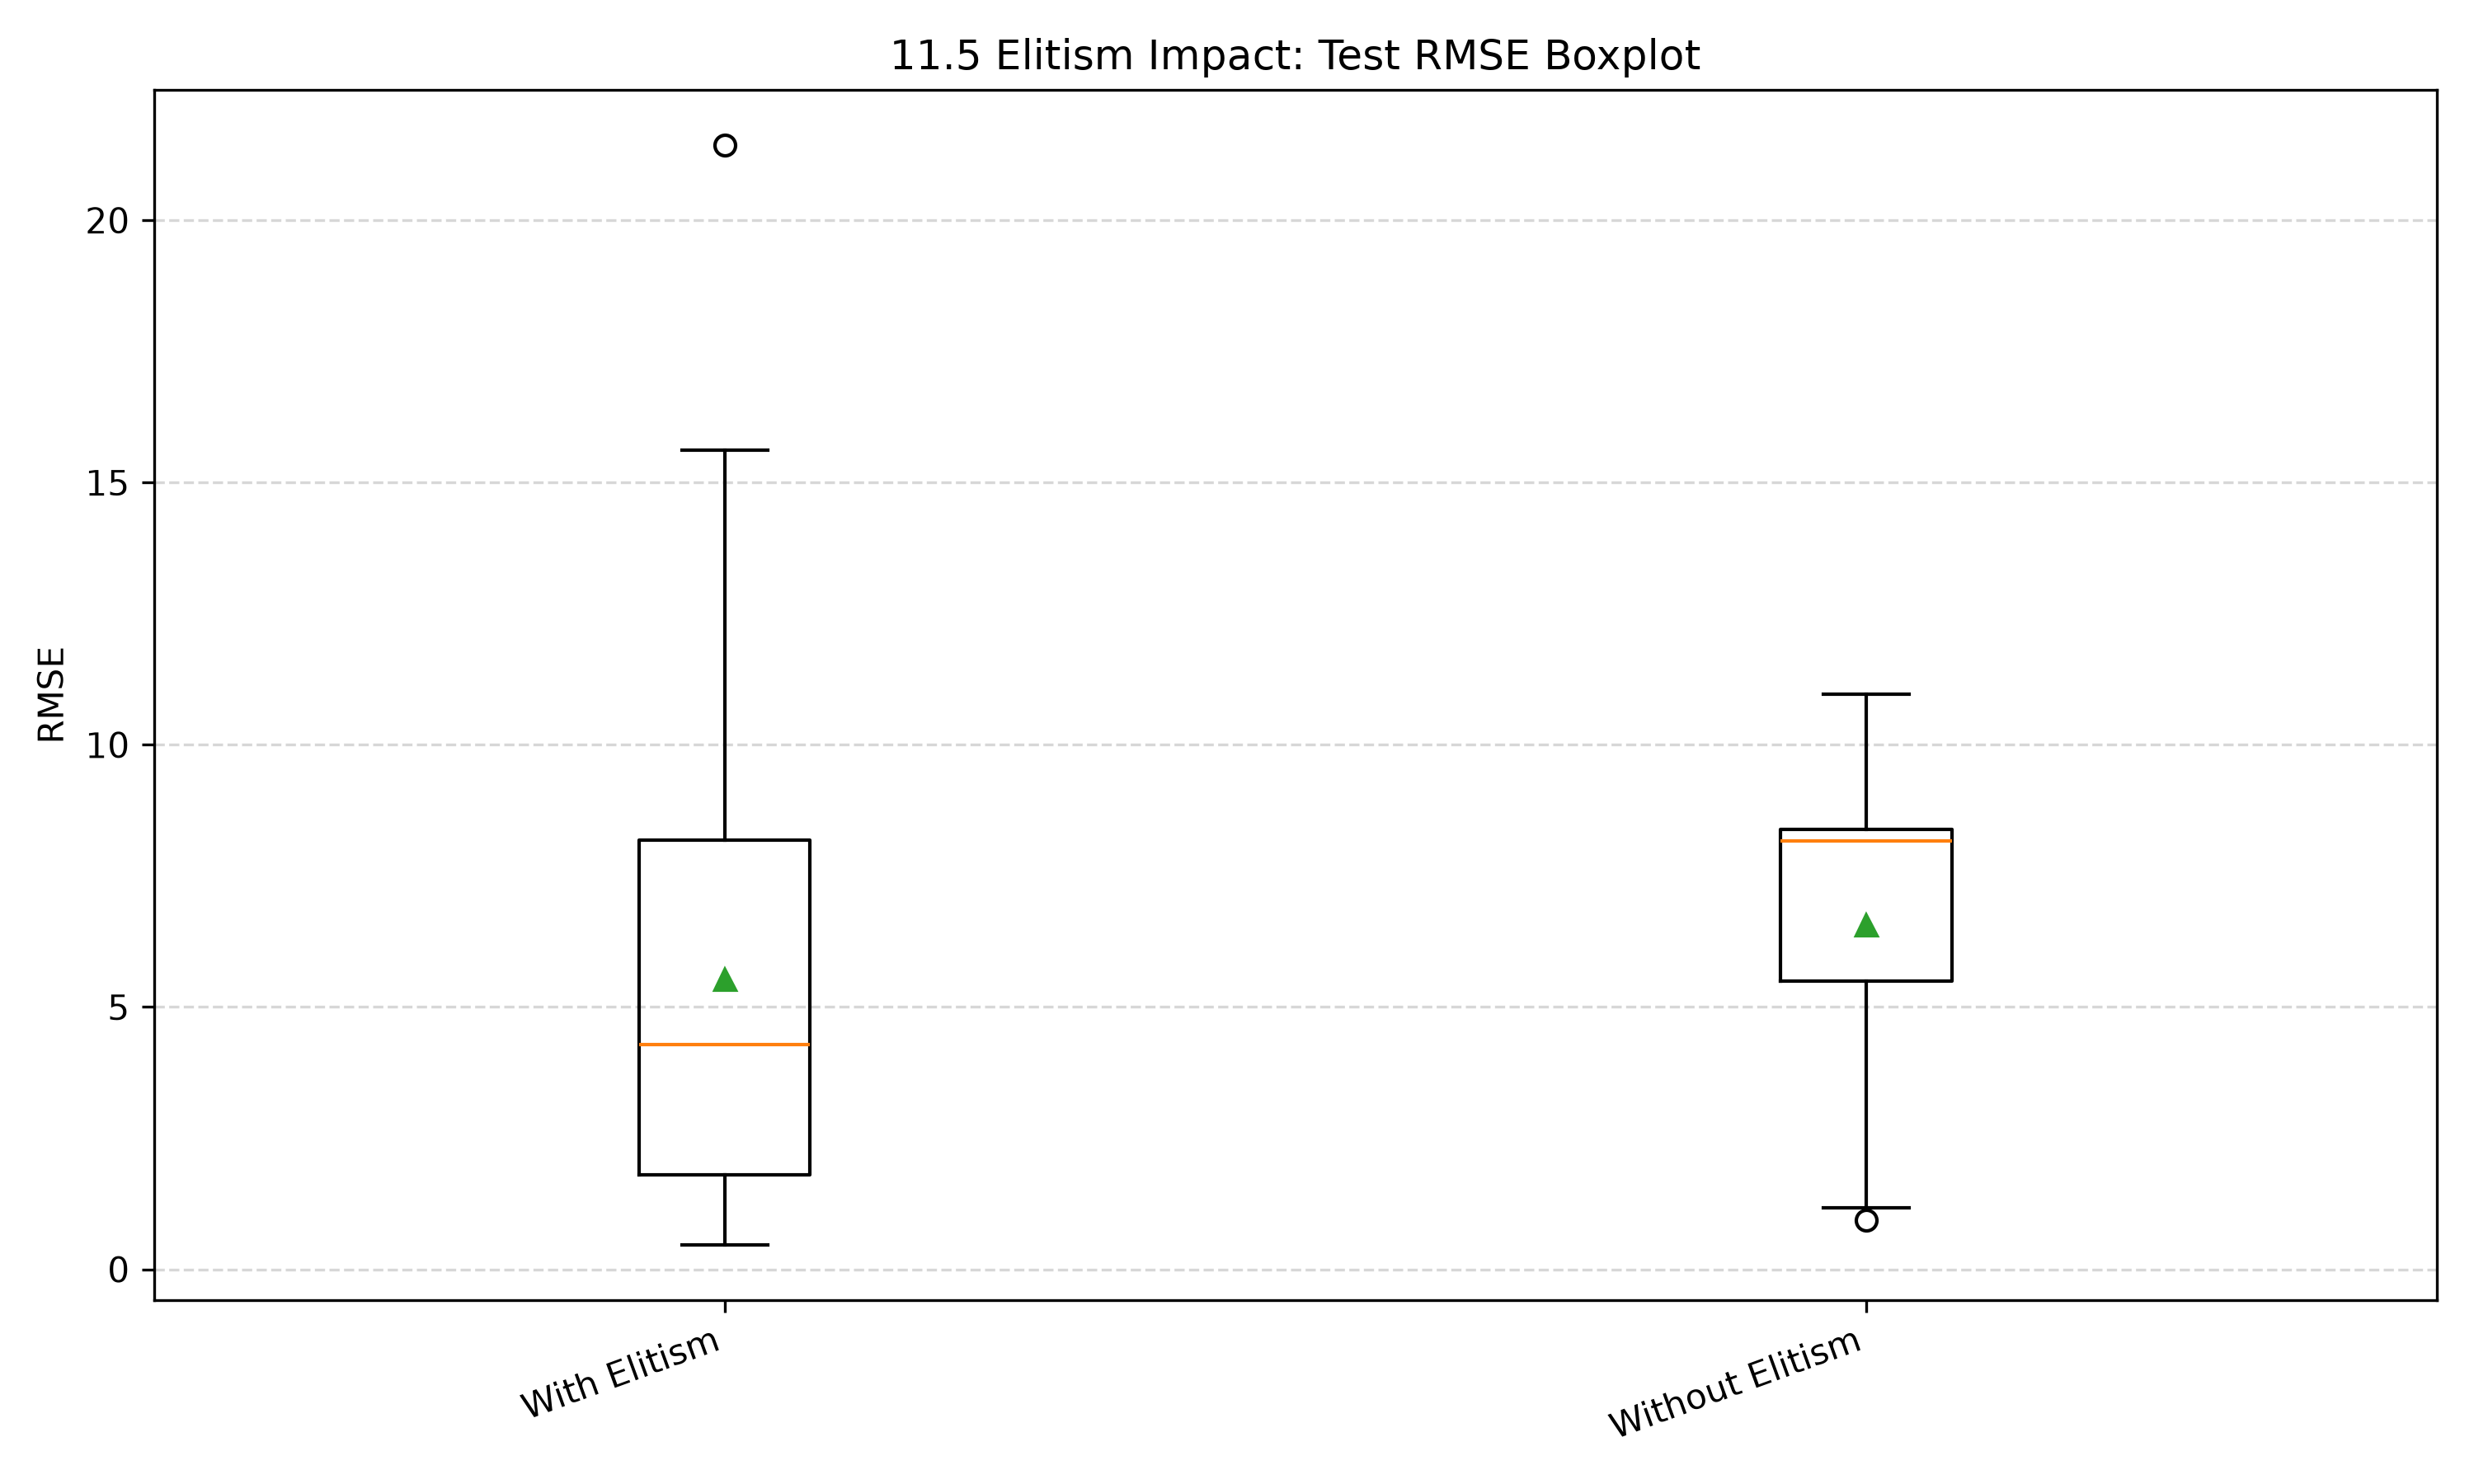
\includegraphics[width=\linewidth]{elitism_test_boxplot.png}
  \end{subfigure}
  \caption{Convergência e RMSE de teste com e sem elitismo.}
  \label{fig:f1_elitismo}
\end{figure}

Sem elitismo, o RMSE de treino piora $33\%$ e a mediana de teste quase dobra
($4.28\to8.16$), como mostram a \cref{tab:f1_elitismo} e a
\cref{fig:f1_elitismo}. Como cerca de $89\%$ dos cruzamentos pioram o melhor
pai, a melhor solução é frequentemente destruída, e a curva do melhor
indivíduo deixa de ser monotônica. As árvores também crescem
($46.5\to54.3$ nós), o que é compatível com a hipótese de \emph{bloat}
defensivo: árvores maiores, com mais \emph{introns}, sobrevivem melhor a
operadores destrutivos~\cite{langdon1997fitness}. O teste de Mann--Whitney
não acusa diferença significativa ($p=0.158$), pois a ausência de elitismo
também reduz a cauda superior (máximo de $10.97$).

% -----------------------------------------------------------------------------
\subsubsection{\emph{Bloating}}
\label{sec:f1_bloat}

\paragraph{Forma simples de medir.} Uma forma otimizada para identificar a presenta de bloat,
que foi escolhida é, registrar a cada geração
o tamanho médio da população (em nós), o tamanho do melhor indivíduo e a
profundidade média, e confrontá-los com a variação do melhor erro. Há
\emph{bloat} quando o tamanho cresce enquanto o erro estagna, isto é,
$\frac{d\,\overline{\text{tam}}}{dt}>0$ com
$\frac{d\,\text{RMSE}^{*}}{dt}\approx0$. Um indicador escalar útil é o fator
de inchaço $\overline{\text{tam}}_{\text{final}}/\overline{\text{tam}}_{G0}$.

\begin{table}[htbp]
  \centering
  \caption{Indicadores de \emph{bloating} na Fase~1.}
  \label{tab:f1_bloat}
  \small
  \begin{tabular}{@{}lccccc@{}}
    \toprule
    Configuração & Tam. médio (G0 $\to$ final) & Fator & Tam. melhor & RMSE teste & Mediana \\
    \midrule
    \code{synth1}, prof.~7, 100 ger.  & $26.2 \to 50.5$  & $1.93\times$ & $46.5 \pm 17.5$ & $5.52 \pm 4.89$ & 4.28 \\
    \code{synth1}, prof.~10, 100 ger. & $130.7 \to 70.2$ & ---          & $64.4 \pm 25.2$ & $4.82 \pm 4.23$ & 2.38 \\
    \code{synth1}, prof.~7, 500 ger.  & $26.2 \to 66.4$  & $2.53\times$ & $64.2 \pm 21.7$ & $3.33 \pm 4.74$ & 1.33 \\
    \code{concrete1}, prof.~7         & $26.2 \to 72.3$  & $2.76\times$ & $74.1 \pm 27.2$ & $11.97 \pm 1.51$ & 11.65 \\
    \bottomrule
  \end{tabular}
\end{table}

\begin{figure}[htbp]
  \centering
  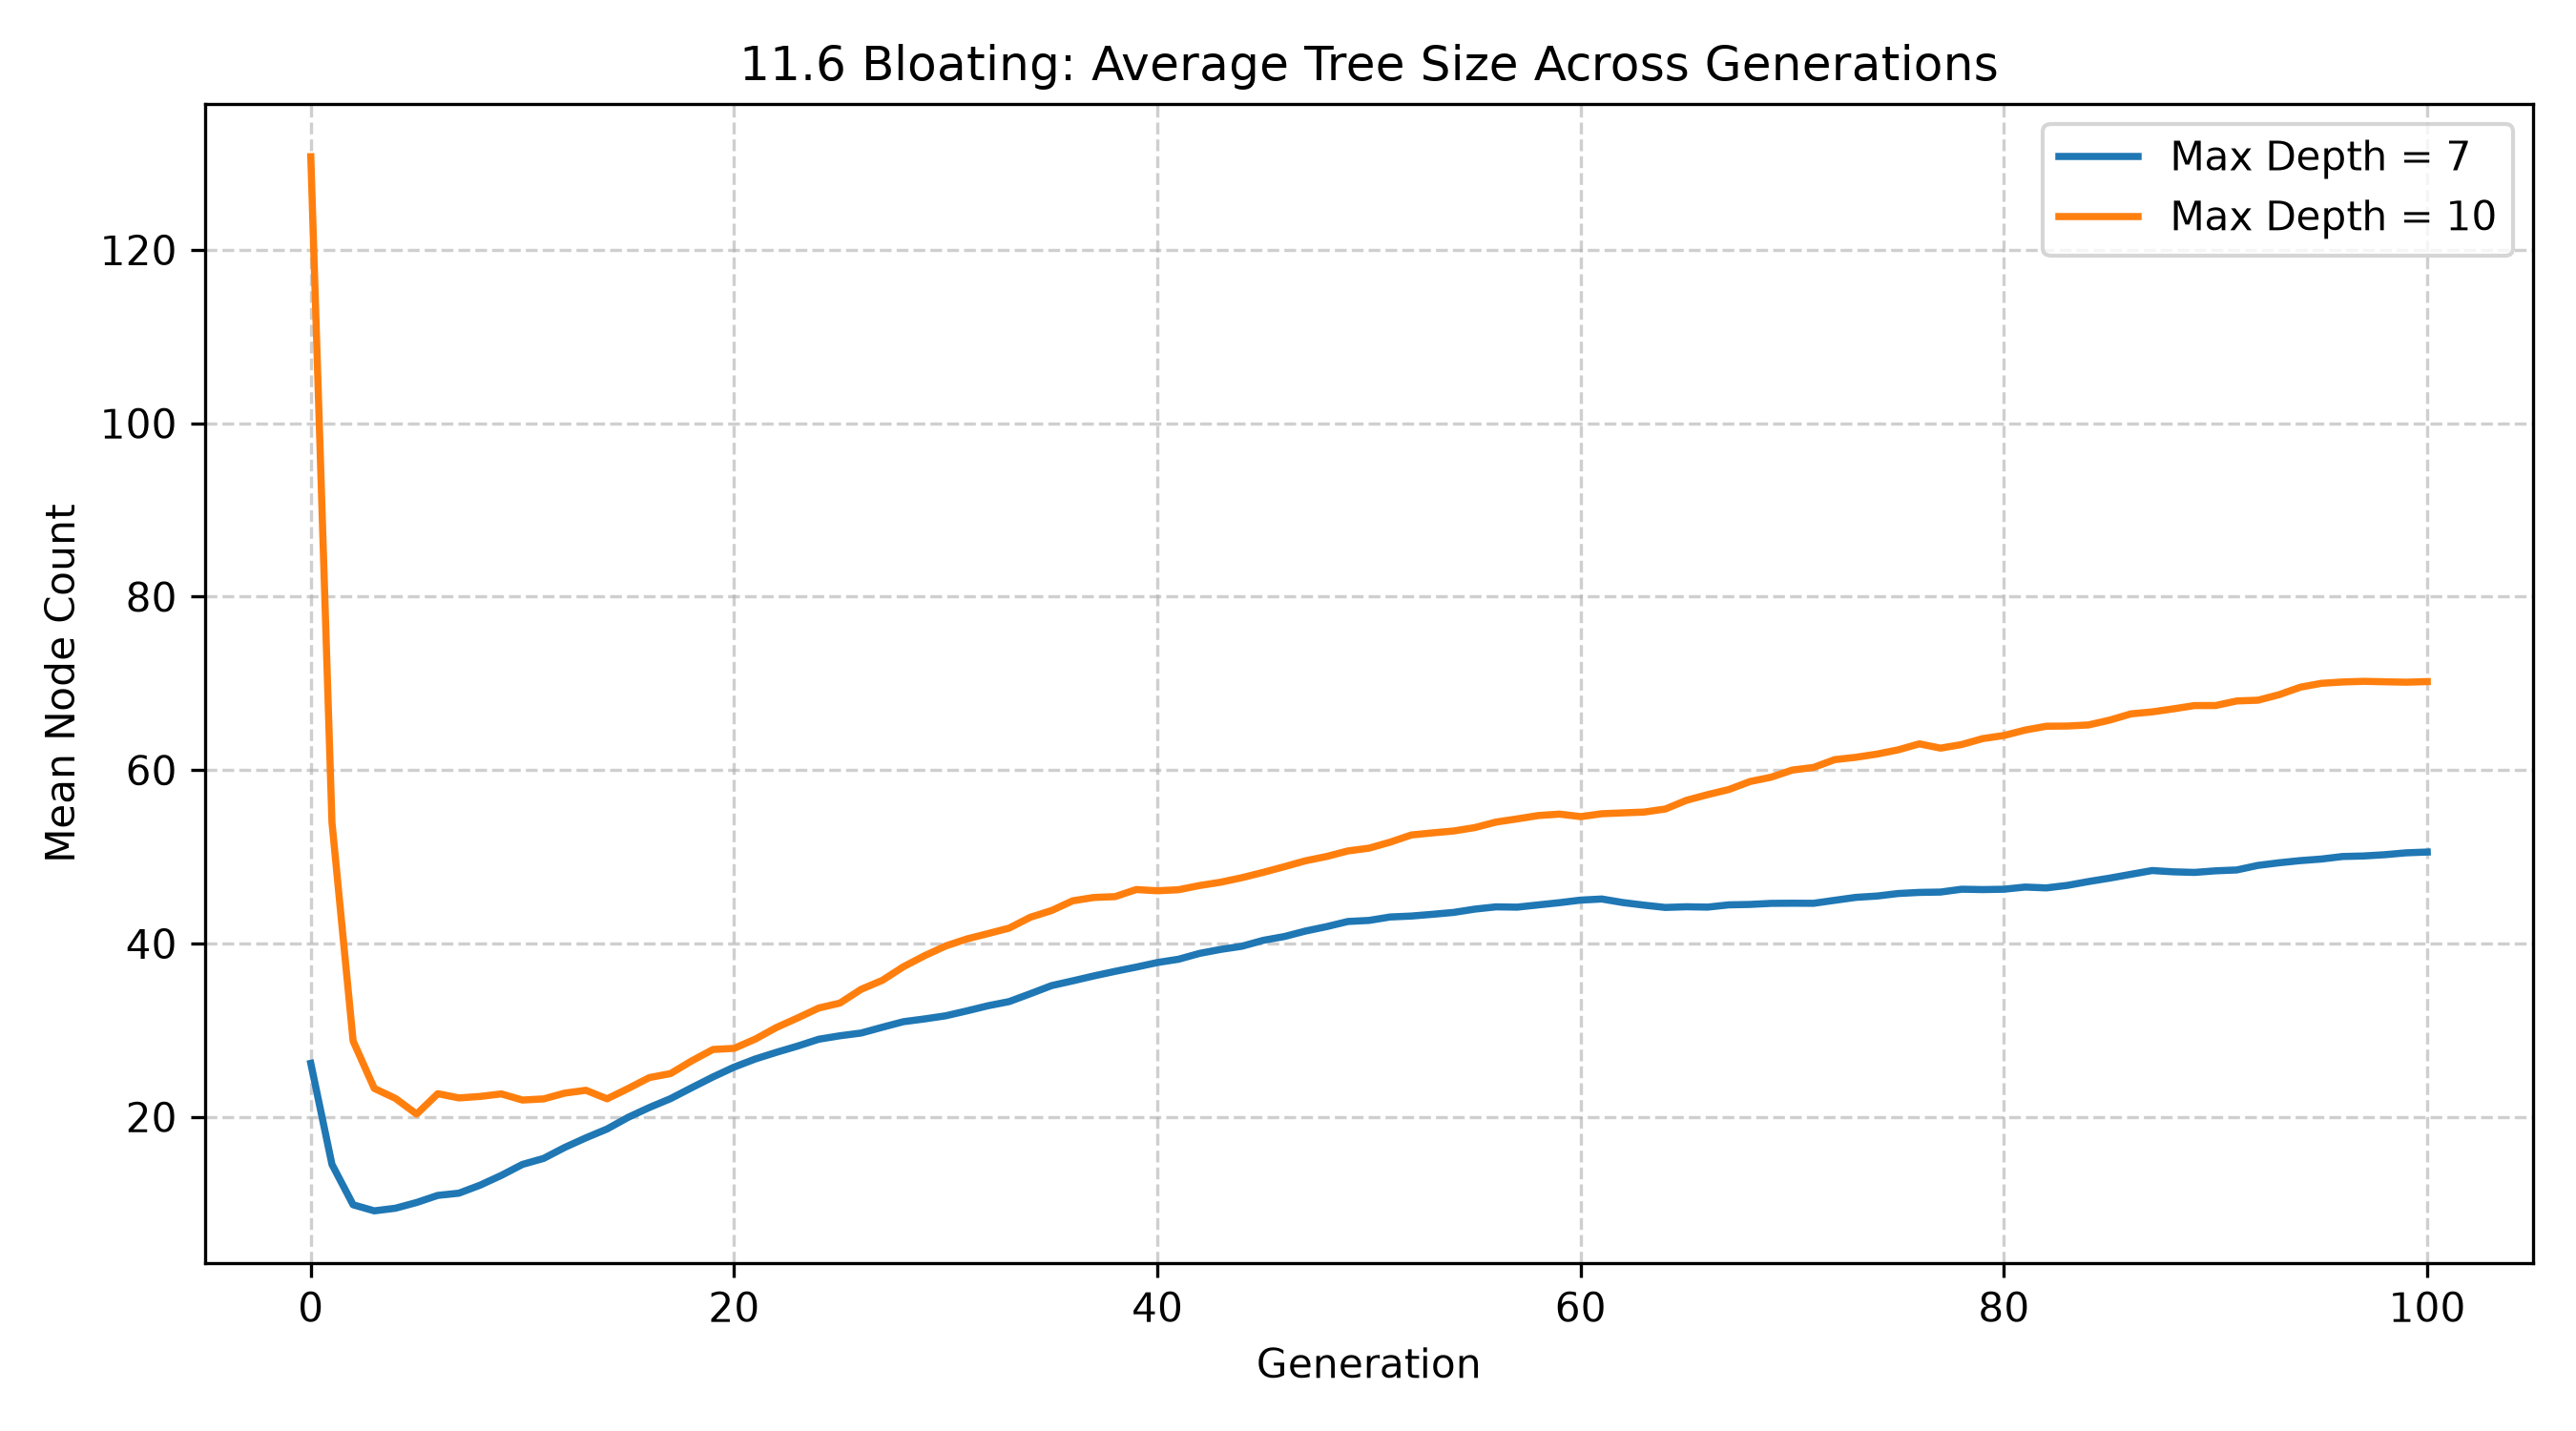
\includegraphics[width=0.75\linewidth]{bloating_depth_comparison.png}
  \caption{Evolução do tamanho médio da população com profundidade máxima 7 e 10.}
  \label{fig:f1_bloat}
\end{figure}

A \cref{tab:f1_bloat} e a \cref{fig:f1_bloat} mostram que o tamanho médio 
dobra em 100 gerações e cresce $2.5\times$ em 500 gerações, enquanto o
erro de treino praticamente não melhora depois da geração~80. Relaxar a
profundidade de 7 para 10 aumenta o tamanho do melhor indivíduo em $38\%$
($46.5\to64.4$ nós), sem ganho significativo de teste ($p=0.57$). As
expressões finais contêm \emph{introns} evidentes (por exemplo,
$x_0-x_0$ e $x_0/x_0$; ver \cref{app:expressoes}), por tanto, o limite de profundidade 7
funciona como regularizador estrutural, mas \textbf{não impede} o
\emph{bloat}.

% -----------------------------------------------------------------------------
\subsubsection{Replicação no \code{synth2} e no \code{concrete1}}
\label{sec:f1_replicacao}

\begin{table}[htbp]
  \centering
  \caption{Replicação da configuração da Fase~1 (torneio $k=2$, $\pc=0.9$,
           $\pmut=0.05$) nas demais bases.}
  \label{tab:f1_replicacao}
  \small
  \begin{tabular}{@{}lcccccc@{}}
    \toprule
    Base & RMSE treino & RMSE teste & Mediana & Máx. teste & Tam. melhor & $R^2_{\text{teste}}$ \\
    \midrule
    \code{synth1}               & $3.69 \pm 2.19$  & $5.52 \pm 4.89$   & 4.28  & 21.44  & $46.5 \pm 17.5$ & 0.95 \\
    \code{synth2}               & $2.66 \pm 0.38$  & $24.97 \pm 80.39$ & 3.47  & \textbf{415.26} & $48.0 \pm 11.6$ & $<0$ \\
    \code{concrete1} (bruto)    & $14.28 \pm 1.36$ & $13.97 \pm 1.44$  & 13.36 & 17.82  & $41.9 \pm 20.5$ & 0.26 \\
    \code{concrete1} (z-score)  & $12.39 \pm 1.45$ & $11.97 \pm 1.51$  & 11.65 & 16.67  & $74.1 \pm 27.2$ & 0.46 \\
    \bottomrule
  \end{tabular}
\end{table}

\begin{figure}[htbp]
  \centering
  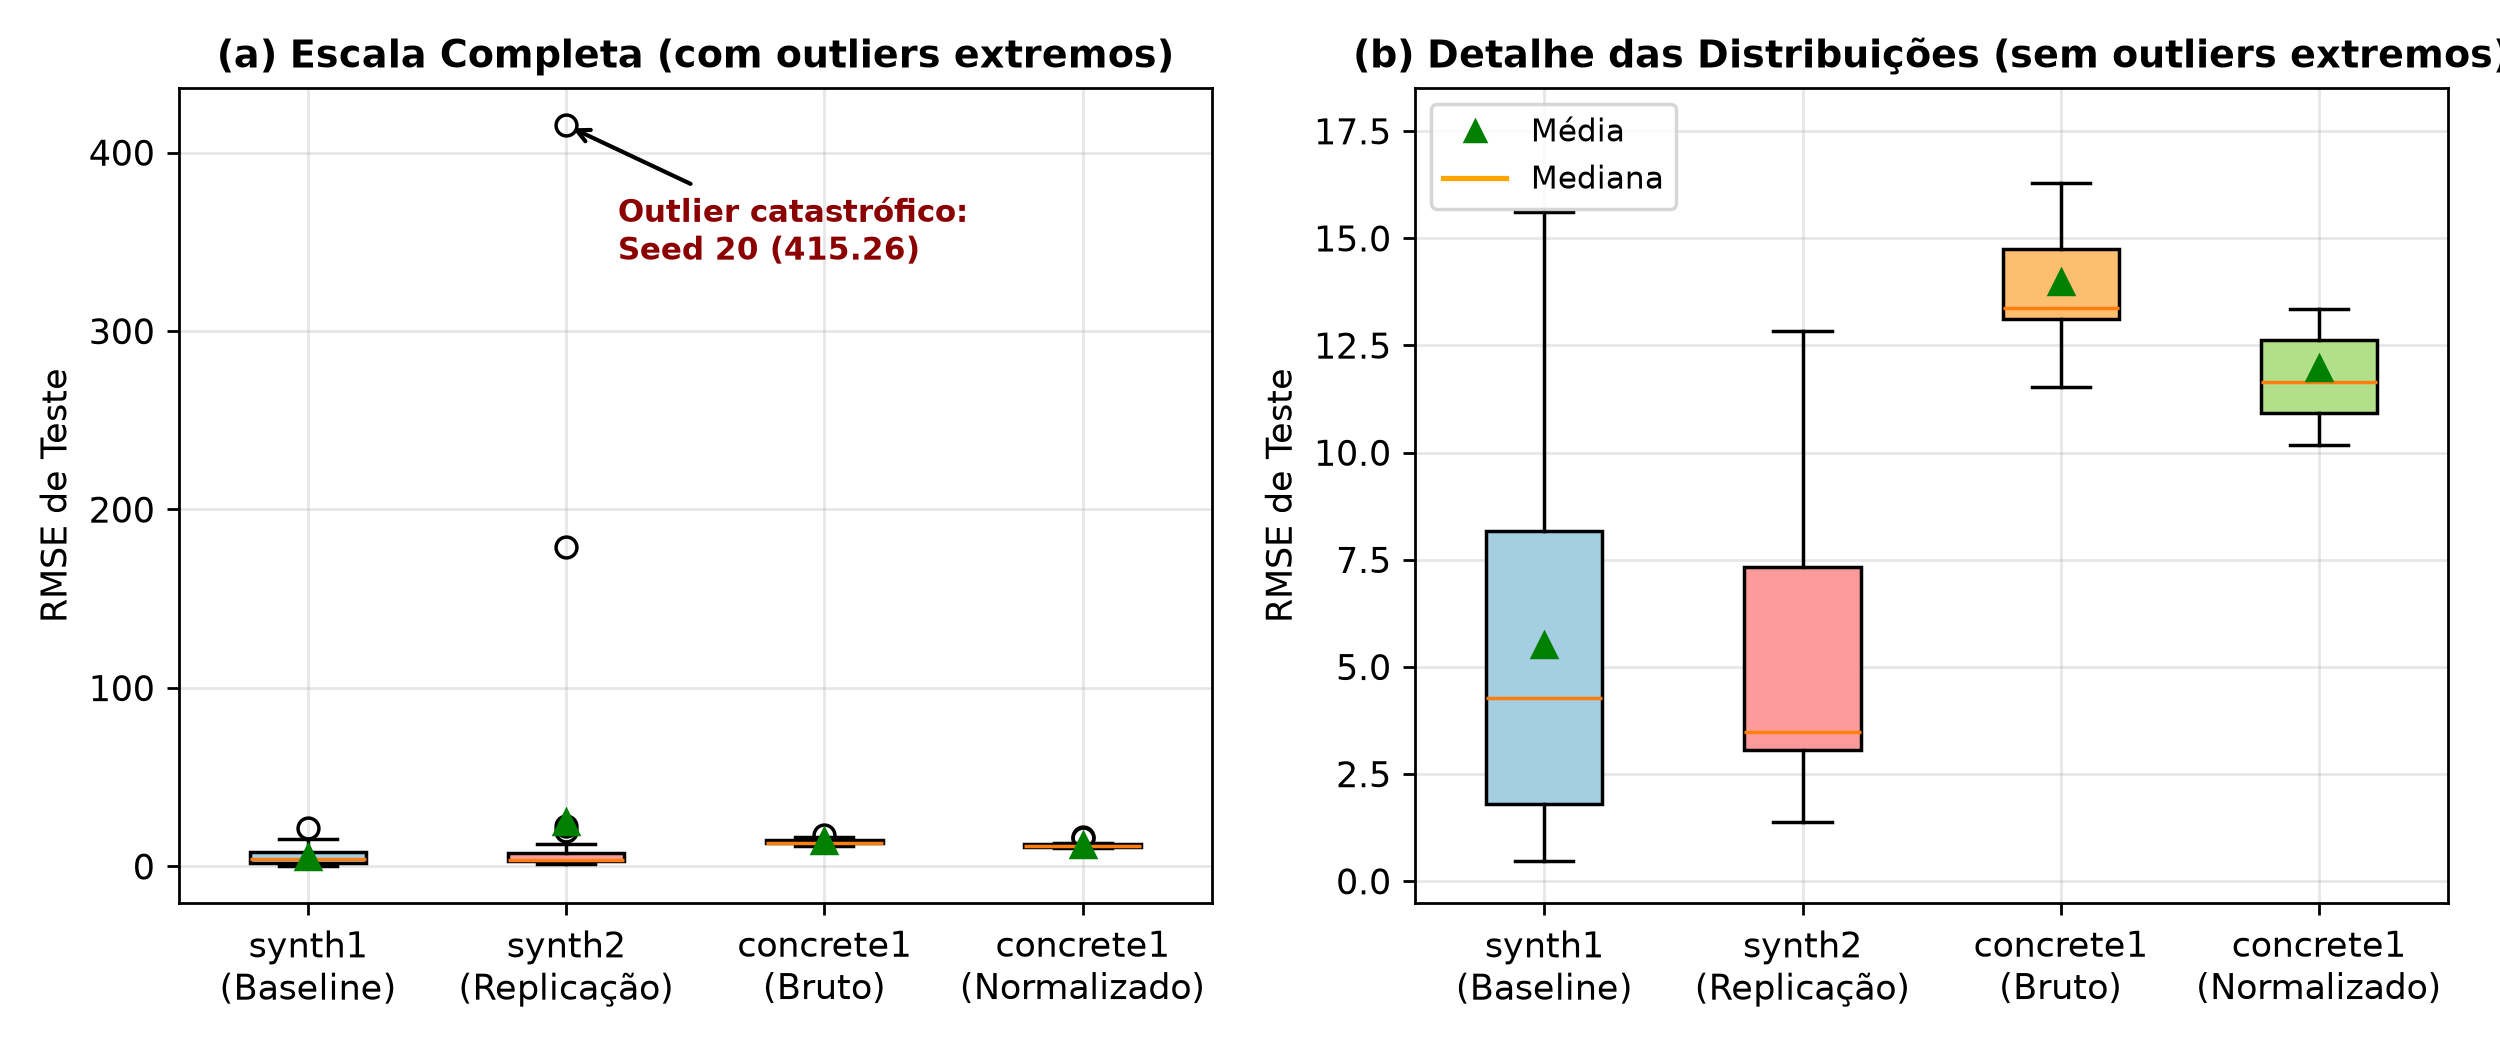
\includegraphics[width=\linewidth]{replication_all_datasets_two_panels.png}
  \caption{Desempenho da replicação da Fase~1 nas três bases (RMSE de teste, 30 execuções).
           O painel (a) exibe a escala completa, destacando os \emph{outliers} catastróficos
           do \code{synth2} decorrentes da divisão protegida clássica. O painel (b) apresenta
           o detalhe das distribuições (com corte de \emph{outliers} extremos fora de $[-0.5, 18.5]$),
           tornando claramente visíveis as medianas (linhas laranjas), médias (triângulos verdes)
           e a dispersão interquartil de todas as bases.}
  \label{fig:f1_replicacao}
\end{figure}

A replicação (\cref{tab:f1_replicacao,fig:f1_replicacao}) revelou
comportamentos qualitativamente diferentes entre as bases:

\begin{itemize}
  \item \textbf{\code{synth2}: sobreajuste catastrófico fora da amostra.}
        Conforme ilustrado no painel~(a) da \cref{fig:f1_replicacao}, embora o
        erro de treino seja baixo e estável ($2.66\pm0.38$), o erro de teste
        explode em 6 das 30 execuções (RMSE $>10$), culminando no valor extremo
        de $415.26$ na semente~20 (e $179.3$ na semente~21). Essa distorção
        comprime visualmente as caixas das demais bases. A inspeção analítica
        mostra que as expressões geraram divisões cujo denominador se aproxima
        de zero \emph{entre} os pontos de treino (ex.: $x_0/(x_0+x_1)$, que se
        anula sobre a reta $x_0 = -x_1$). Como a divisão de Koza (\cref{eq:div})
        só atua para $|b| < 10^{-6}$, qualquer denominador pequeno superior a
        esse limiar produz assíntotas gigantescas no teste.
  \item \textbf{\code{concrete1}: subajuste estrutural e ganho por normalização.}
        Graças ao painel detalhado~(b) da \cref{fig:f1_replicacao}, constata-se
        nitidamente que os erros de treino e teste são muito próximos ($12.4$ e
        $12.0$), descartando sobreajuste, mas indicando subajuste
        ($R^2 \approx 0.46$). Observa-se com clareza o benefício da
        normalização \emph{z-score} dos atributos de entrada frente aos dados
        brutos: a mediana cai de $13.36$ para $11.65$ e a média de $13.97$
        para $11.97$, com ganho estatisticamente significativo
        ($U = 786.0$, $p = 7.04\times10^{-7}$). Contudo, as árvores incham até
        74 nós para sintetizar a magnitude elevada da resposta ($\bar{y} \approx 35.8$); ver
        \cref{app:expressoes}.
  \item \textbf{\code{synth1}: consistência com gap moderado.} O painel~(b)
        evidencia que a distribuição do \code{synth1} concentra a maioria das
        sementes na faixa de 0 a 8 (mediana $4.28$), apresentando razão
        mediana teste/treino de $1.34$, plenamente compatível com o reduzido
        volume amostral de treino (60 amostras).
\end{itemize}

% -----------------------------------------------------------------------------
\subsubsection{Síntese da Fase 1 e questões em aberto}
\label{sec:f1_sintese}

\begin{table}[htbp]
  \centering
  \caption{Respostas da Fase~1 às questões do enunciado.}
  \label{tab:f1_sintese}
  \small
  \begin{tabularx}{\linewidth}{@{}lX@{}}
    \toprule
    Questão & Resposta da Fase~1 \\
    \midrule
    População/gerações & 100/100: saturação na geração $\approx80$; mais orçamento ajuda, preferencialmente em população. \\
    Seleção            & $\eps$-lexicase é o único fator significativo ($p=4.1\times10^{-6}$); roleta $\approx$ torneio $k=2$; $k=3$ provoca convergência prematura. \\
    $\pc$ e $\pmut$    & \emph{Crossover} destrutivo em 89\% dos casos (em relação ao melhor pai); ótimo intermediário ($\pc\approx0.7$, $\pmut\approx0.1$) indicado, mas não testado em conjunto. \\
    Elitismo           & Necessário: sem ele, a mediana do teste dobra e as árvores crescem. \\
    \emph{Bloating}    & Medido pelo tamanho médio/melhor ao longo das gerações; fator de $1.9\times$ a $2.8\times$; o limite de profundidade não o impede. \\
    Treino $\times$ teste & \code{synth2}: explosões fora da amostra; \code{concrete1}: subajuste ($R^2\approx0.46$). \\
    \bottomrule
  \end{tabularx}
\end{table}

A \cref{tab:f1_sintese} resume as respostas. A Fase~1 deixou cinco sintomas
sem explicação mecanística, que motivam a Fase~2:
\textbf{(S1)}~explosões assintóticas no \code{synth2};
\textbf{(S2)}~\emph{crossover} destrutivo e ótimo de operadores não validado;
\textbf{(S3)}~10--27\% de clones por geração, mesmo com $\eps$-lexicase no
final da evolução;
\textbf{(S4)}~crescimento das árvores com \emph{introns}; e
\textbf{(S5)}~subajuste estrutural no \code{concrete1}. Além disso, a
$\eps$-lexicase só havia sido avaliada no \code{synth1}.
